%Auteur : Nicolas Englebert
\documentclass[british,french,11pt, a4paper, openany]{book}

% Règles de bonne pratiques :
% https://fr.wikibooks.org/wiki/LaTeX/Gestion_des_gros_documents

%%%%%%%%%%%%%%%%%
%%% Packages %%%
%%%%%%%%%%%%%%%%

%%% Compatibilité %%%
\begingroup\expandafter\expandafter\expandafter\endgroup
\expandafter\ifx\csname IncludeInRelease\endcsname\relax
\usepackage{fixltx2e}
\fi 					% Si version LaTeX < 2015, inclut un fix.

%%% Général %%%
\usepackage[utf8]{inputenc}
\usepackage{babel}
\usepackage{lmodern}
\usepackage[T1]{fontenc}
\addto\extrasfrench{\sisetup{locale = FR,detect-all}} % Switch siunitx en fonction de la langue babel :)
\addto\extrasbritish{\sisetup{locale = UK,detect-all}}
\usepackage{courier}
\usepackage{graphicx}
%\usepackage{cancel}

%%% Tableau %%%
%\usepackage{tabularx} %Permet d'auto dimensionner les tableaux



%%% Bibliographie %%%
%\usepackage[style=alphabetic,backend=biber]{biblatex}
\usepackage[autostyle]{csquotes}
%\DeclareNameAlias{sortname}{last-first}
%\DeclareFieldFormat{url}{\space\url{#1}}
%\DeclareNameAlias{labelname}{last-first}
%\addbibresource{sample.bib}


%%% Graphiques %%%
%\usepackage{tikz}
%\usepackage{pgfplots}
%\usepackage{circuitikz}

%%% Mise en page %%%
\usepackage{mathtools}
\usepackage{amssymb}
\usepackage{bbm}
\usepackage{amsthm}
%\usepackage[tt]{titlepic}% Centre le titre
%\usepackage{fancyhdr}   % Permet de modifier l'entête & footer
\usepackage{caption}     % Permet d'ajouter des légendes en images sans les mettre en float + dans la marge + ref vers le haut de l'envirronement
\usepackage{wrapfig}
\usepackage{fullpage}
%\usepackage{multicol}   % pour les liste sur plusieurs colonnes
%\usepackage{subfigure}  % alligne deux images cote a cote
\usepackage{float}      %permet de mettre du texte entre les figures grace a [H]. Génial! 
\usepackage{eso-pic}    % Fond d'écran page de garde
\usepackage{adjustbox}  % Empêche les box de sortir de la page


%%% Math %%%
%\usepackage{delarray} % Belles matrices
\usepackage{siunitx}


%%% Codes %%%
%\usepackage{listings}
%\usepackage[final]{pdfpages} %% Inclusion fichier pdf

%% Reference
\usepackage{hyperref}
%\renewcommand*{\figureautorefname}{fig.}
%\def\appendixautorefname{annexe}
%\def\tableautorefname{tab.}
%\renewcommand*{\chapterautorefname}{ch.}
%\newcommand{\subfigureautorefname}{\figureautorefname}



%%%%%%%%%%%%%%%%%
%%% Commandes %%%
%%%%%%%%%%%%%%%%%

%%% Physique %%%
\newcommand{\cst}{\text{cst}}
\newcommand{\D}{\partial}
\newcommand{\E}{\vec E}
\newcommand{\B}{\vec B}
\newcommand{\F}{\vec F}
\newcommand{\modu}[1]{|$#1$|}

%%% Math %%%
\newcommand{\oiint}{\int\!\!\!\!\!\!\! \:\!\subset\!\!\supset\!\!\!\!\!\!\!\int}
\newcommand{\rot}{\operatorname{\vec{rot}}}
\newcommand{\divv}{\operatorname{div}}
\newcommand{\phas}[1]{\underline{#1}}
\newcommand{\RE}{\text{Re}}
\newcommand{\ft}{\overset{\mathcal{F}}{\longleftrightarrow}}
\newcommand{\lt}{\overset{\mathcal{L}}{\longleftrightarrow}}
\newcommand{\DS}{\displaystyle}
\newcommand{\Tr}{\operatorname{Tr}}



%% Box
\shorthandon{:}
\newcommand{\theor}[1]{\adjustbox{minipage=\linewidth-2\fboxsep-2\fboxrule,fbox}{\textsc{\iflanguage{british}{Theorem}{Théorème}: }#1}}
\newcommand{\defi}[1]{\adjustbox{minipage=\linewidth-2\fboxsep-2\fboxrule,fbox}{\textsc{\iflanguage{british}{Definition}{Définition}: }#1}}
\newcommand{\lemme}[1]{\adjustbox{minipage=\linewidth-2\fboxsep-2\fboxrule,fbox}{\textsc{\iflanguage{british}{Lemma}{Lemme}: }#1}}
\newcommand{\prop}[1]{\adjustbox{minipage=\linewidth-2\fboxsep-2\fboxrule,fbox}{\textsc{\iflanguage{british}{Property}{Propriété}}\\ #1}}
\newcommand{\proposition}[1]{\adjustbox{minipage=\linewidth-2\fboxsep-2\fboxrule,fbox}{\textsc{Proposition}\\#1}}
\newcommand{\cadre}[1]{\adjustbox{minipage=\linewidth-2\fboxsep-2\fboxrule,fbox}{#1}}
\newcommand{\retenir}[1]{\adjustbox{minipage=\linewidth-2\fboxsep-2\fboxrule,fbox}{\textbf{\textit{\textsc{\iflanguage{british}{To remember}{À retenir}}: }}#1}}

\newcommand{\corollaire}[1]{\bigbreak\begin{tabular}{||c}
	\begin{minipage}{\textwidth}
		\textsc{\iflanguage{british}{Corollary}{Corollaire}: } \textit{#1}
	\end{minipage}
	\end{tabular}}
\newcommand{\exemple}[1]{\bigbreak\begin{tabular}{|c}
	\begin{minipage}{\textwidth}
		\textsc{\iflanguage{british}{Example}{Exemple}: } #1
	\end{minipage}%
	\end{tabular}}%
\shorthandoff{:}
    

%\pagestyle{headings} % Titre du ch et numéro page dans l'entete
%\renewcommand{\proofname}{Démonstration}
%\addto\captionsfrench{\def\tablename{Tableau}}


%%% Background %%%
\newcommand\BackgroundPic{%
	\put(0,0){%
		\parbox[b][\paperheight]{\paperwidth}{%
			\vfill
			\centering
			\includegraphics[width=\paperwidth,height=\paperheight,%
			keepaspectratio]{../../Builder/ulb.jpg}%
			\vfill
}}}

%%% Annexes Cedu %%%
%\usepackage{calrsfs}
%\DeclareMathAlphabet{\pazocal}{OMS}{zplm}{m}{n}
\usepackage{fourier-orns}

\setlength{\parindent}{0pt} 

%%% Attributs %%%
\newcommand*{\NomduCours}[2]{\def\cours{#1}\def\memo{#2}}
\newcommand*{\annee}[2]{\def\adebut{#1}\def\afin{#2}}

\newcounter{auteurcnt}
\newcommand\addauteur[2]{%
	\stepcounter{auteurcnt}%
	\csdef{auteur\theauteurcnt}{\mbox{#1~\textsc{#2}}}}
\newcommand\getauteur[1]{%
	\csuse{auteur#1}}

\newcounter{illustrateurcnt}
\newcommand\addillustrateur[2]{%
	\stepcounter{illustrateurcnt}%
	\csdef{illustrateur\theillustrateurcnt}{\mbox{#1~\textsc{#2}}}}
\newcommand\getillustrateur[1]{%
	\csuse{illustrateur#1}}

\newcounter{rappeltheocnt}
\newcommand\addrappeltheo[2]{%
	\stepcounter{rappeltheocnt}%
	\csdef{rappeltheo\therappeltheocnt}{\mbox{#1~\textsc{#2}}}}
\newcommand\getrappeltheo[1]{%
	\csuse{rappeltheo#1}}

\newcounter{professeurcnt}
\newcommand\addprofesseur[2]{%
	\stepcounter{professeurcnt}%
	\csdef{professeur\theprofesseurcnt}{\mbox{#1~\textsc{#2}}}}
\newcommand\getprofesseur[1]{%
	\csuse{professeur#1}}

\newcounter{iter}
%\usepackage{ulem}
%Typique Phys
\usepackage{soul}
\usepackage{../../Builder/preambule}
\usepackage{cancel,physics}
% Attributs
\NomduCours{Quantum Information and Comutation}{INFO-H514}
\addauteur{Nicolas}{Englebert}
\addprofesseur{Nicolas}{Cerf}
\annee{2017}{2018}


% Document
\begin{document}
\def\equationautorefname~#1\null{%
	(#1)\null
}
%%%%%%%%%%%%%%%%%
% Préliminaires %
%%%%%%%%%%%%%%%%%
\frontmatter
\AddToShipoutPicture*{\BackgroundPic}

\begin{titlepage}
	\begin{center}	
			
		\newcommand{\HRule}{\rule{\linewidth}{0.5mm}}   			            %Titre en gros
		\includegraphics[width=0.55\textwidth]{../../Builder/titlepage/logo.pdf}~\\[1cm]				%Logo
			
			\textsc{\LARGE Université Libre de Bruxelles}\\[1.5cm]
			\textsc{\Large \iflanguage{british}{Summary}{Synthèse}}\\[0.5cm]
			
			\HRule \\[0.4cm]
			{ \huge \bfseries \cours \ \\\memo \\[0.4cm] }
			
			
			\HRule \\[1.5cm]
			\begin{minipage}[t]{0.6\textwidth}
				\begin{flushleft}%\large
					\emph{\iflanguage{british}{Author}{Auteur}\ifnum\theauteurcnt>1 s\fi:}\\
					\whileboolexpr
					{ test {\ifnumcomp{\value{iter}}{<}{\theauteurcnt}} }%
					{\stepcounter{iter}\getauteur{\theiter}\\}
					\setcounter{iter}{0}%
					\ifnum\theillustrateurcnt>0%
					\ \\
					\emph{Illustrations:}\\
					\whileboolexpr
					{ test {\ifnumcomp{\value{iter}}{<}{\theillustrateurcnt}} }%
					{\stepcounter{iter}\getillustrateur{\theiter}\\}%
					\setcounter{iter}{0}%
					\fi%
					\ifnum\therappeltheocnt>0%
					\ \\
					\emph{\iflanguage{british}{Reminders}{Rappels théoriques}:}\\
					\whileboolexpr
					{ test {\ifnumcomp{\value{iter}}{<}{\therappeltheocnt}} }%
					{\stepcounter{iter}\getrappeltheo{\theiter}\\}%
					\setcounter{iter}{0}%
					\fi%
				\end{flushleft}
			\end{minipage}%
			\begin{minipage}[t]{0.25\textwidth}
				%\begin{flushright}
				%\large
				\emph{\iflanguage{british}{Professor}{Professeur}\ifnum\theprofesseurcnt>1 s\fi:}
				\whileboolexpr
				{ test {\ifnumcomp{\value{iter}}{<}{\theprofesseurcnt}} }%
				{\\ \stepcounter{iter}\getprofesseur{\theiter}}%
				\setcounter{iter}{0}%
				%\end{flushright}
			\end{minipage}
			
			\vfill
			
			% Bottom of the page
			{\large \iflanguage{british}{Year}{Année} \adebut~-~\afin}
			
		\end{center}
	\end{titlepage}

\ \\[2cm]
{\Huge \bfseries Appel à contribution}\\[5mm]
\subsection*{Synthèse Open Source}
\begin{wrapfigure}[5]{l}{4.5cm}
	\includegraphics[scale=0.5]{../../Builder/git.png}
\end{wrapfigure}
Ce document est grandement inspiré de l’excellent cours donné 
par \ifnum\theprofesseurcnt=1 \getprofesseur{1} \else\whileboolexpr
{ test {\ifnumcomp{\value{iter}}{<}{\theprofesseurcnt-2}} }%
{\stepcounter{iter}\getprofesseur{\theiter}, }%
\stepcounter{iter}\getprofesseur{\theiter} et \stepcounter{iter}\getprofesseur{\theiter} \fi%
 à l’EPB (École Polytechnique de Bruxelles), faculté de l’ULB (Université 
Libre de Bruxelles). Il est écrit par les auteurs susnommés avec l’aide de tous les autres étudiants 
et votre aide est la bienvenue ! En effet, il y a toujours moyen de l’améliorer surtout que si le 
cours change, la synthèse doit être changée en conséquence. On peut retrouver le code source à l’adresse 
suivante
\begin{center}
	\url{https://github.com/nenglebert/Syntheses}
\end{center}\bigskip
Pour contribuer à cette synthèse, il vous suffira de créer un compte sur \textit{Github.com}. De
légères modifications (petites coquilles, orthographe, ...) peuvent directement être faites sur le
site ! Vous avez vu une petite faute ? Si oui, la corriger de cette façon ne prendra que quelques 
secondes, une bonne raison de le faire ! \bigskip

Pour de plus longues modifications, il est intéressant de disposer des fichiers : il vous 
faudra pour cela installer \LaTeX, mais aussi \textit{git}. Si cela pose problème, nous sommes 
évidemment ouverts à des contributeurs envoyant leur changement par mail ou n’importe quel autre 
moyen.\bigskip

Le lien donné ci-dessus contient aussi un \texttt{README} contenant de plus amples informations, 
vous êtes invités à le lire si vous voulez faire avancer ce projet ! 

\subsection*{Licence Creative Commons}
\begin{wrapfigure}[3]{r}{2.8cm}
	\vspace{-5mm}
	\includegraphics[scale=0.17]{../../Builder/CC}
\end{wrapfigure}
Le contenu de ce document est sous la licence Creative Commons : \textit{Attribution-NonCommercial-ShareAlike 
4.0 International (CC BY-NC-SA 4.0)}. Celle-ci vous autorise à l'exploiter pleinement, compte-
tenu de trois choses :
\begin{enumerate}
	\item \textit{Attribution} ; si vous utilisez/modifiez ce document vous devez signaler le(s) nom(s)
	      de(s) auteur(s).
	\item \textit{Non Commercial} ; interdiction de tirer un profit commercial de l’œuvre sans 
	      autorisation de l'auteur 
	\item \textit{Share alike} ;  partage de l’œuvre, avec obligation de rediffuser selon la même 
	      licence ou une licence similaire
\end{enumerate}
Si vous voulez en savoir plus sur cette licence :
\begin{center}
	\url{http://creativecommons.org/licenses/by-nc-sa/4.0/}
\end{center}

\begin{flushright}
	\textbf{Merci ! }
\end{flushright}
\tableofcontents
%Si abstract, \input ici

%%%%%%%%%%%%%%%%%%%%%
% Contenu principal %
%%%%%%%%%%%%%%%%%%%%%
\mainmatter
\chapter{Interaction des particules chargées avec la matière : considérations de base}
\section{Introduction}
Il existe trois types de rayonnements ionisants (\textit{ionizing radiations})
\begin{enumerate}
\item Les particules chargées
\begin{itemize}
\item Électron, positron, ions, \dots
\end{itemize}
\item Les photons (particules neutres sans masses)
	\begin{itemize}
	\item Les $\gamma$ (origine \textbf{nucléaire})
	\item Les $X$ (origine atomique)
	\end{itemize}
\item Neutrons (particules neutres)
\end{enumerate}
Notons que ce qui fait vraiment la différence entre un $\gamma$ et un $X$ est le mode 
d'émission et non pas l'énergie (conséquence).\\

Pour chacun de ces types de rayonnement, il existe un mécanisme d'interaction particulier
avec la matière\footnote{\textit{Assemblage d'atomes isolés sans interaction entre-eux : 
gaz d'atome}. Il s'agit de la définition de ce cours, qui évoluera au fil des chapitres}. 
\begin{itemize}
\item[$\bullet$] Les particules chargées interagissent par interactions coulombienne 
(noyaux et électrons), les collisions sont donc fréquentes et on peut considérer que 
l'énergie est perdue de façon (quasi-)continue. La particule s'arrête ainsi à distance 
finie dans la matière de sorte à ce qu'on puisse définir un "parcours" (\textit{range}) 
de celle ci  : de tels rayonnements sont \textit{directement} ionisants
\item[$\bullet$] Les particules neutres (pas d'interaction coulombienne) ont une 
probabilité de traverser la matière sans interactions, il n'est donc pas possible de 
définir un range. Elles peuvent par contre déposées de l'énergie à des particules 
chargées qui vont causés une ionisation : de tels rayonnements sont \textit{indirectement} 
ionisants
\end{itemize}
Les interactions d'un rayonnement avec la matière peut modifier l'état du rayonnement 
(absorbé, dévié, \dots) et aussi l'état de la matière (excités, ionisés,\dots).

\newpage
\subsection{Interaction des particules chargées avec la matière}
	\begin{wrapfigure}[7]{l}{6cm}
	\vspace{2mm}
	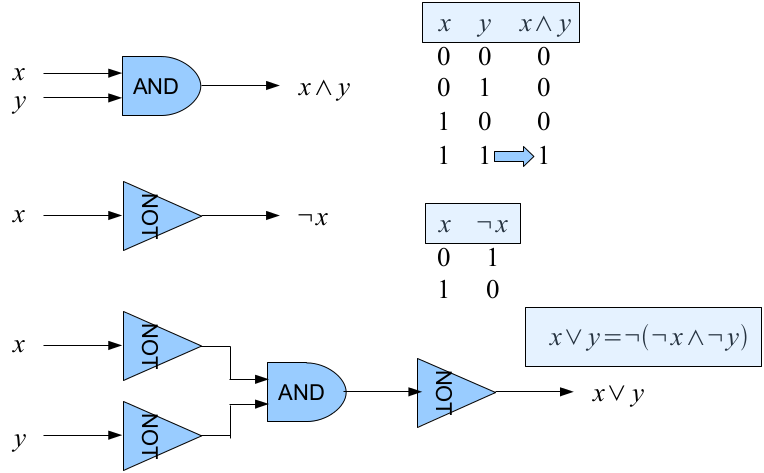
\includegraphics[scale=0.4]{ch1/image1.png}
	\captionof{figure}{Trajectoire d'une particule chargée}
	\end{wrapfigure}
Comme annoncé ci-dessus, les particules chargées subissent des collisions 
coulombiennes\footnote{Les réactions nucléaires sont laissées de côté.} avec :
\begin{description}
\item[Les noyaux (rare)] : cause une importante perte d'énergie et une grande déviation
angulaire
\item[Les électrons (fréquent)] : cause des excitations/ionisations se traduisant par des
faibles pertes d'énergie et déviations angulaires
\end{description}\ \\

	\begin{wrapfigure}[7]{r}{6cm}
	\vspace{-9mm}
	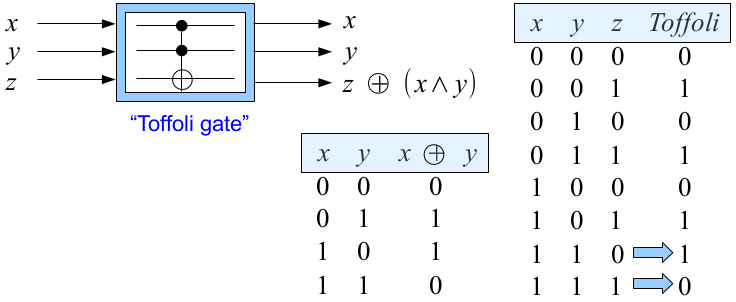
\includegraphics[scale=0.4]{ch1/image2.png}
	\captionof{figure}{ }
	\end{wrapfigure}
Chaque collision cause alors une perte d'énergie $T_j$, causés par un grand nombre de 
projectiles $N$ qui suivent $N$ histoires propres : le nombre de collision étant très 
important, les fluctuations sont faibles et il devient possible de définir des quantités
moyennes.\\

Pour introduire ces valeurs moyennes, il faut avant tout introduire la notion de 
\textbf{section efficace}.\ \\

\cadre{La \textbf{section efficace} est l'aire fictive que doit avoir une particule incidente
pour reproduire la probabilité de collision observée avec une particule cible.}\ \\

	\begin{wrapfigure}[7]{l}{6cm}
	\vspace{-5mm}
	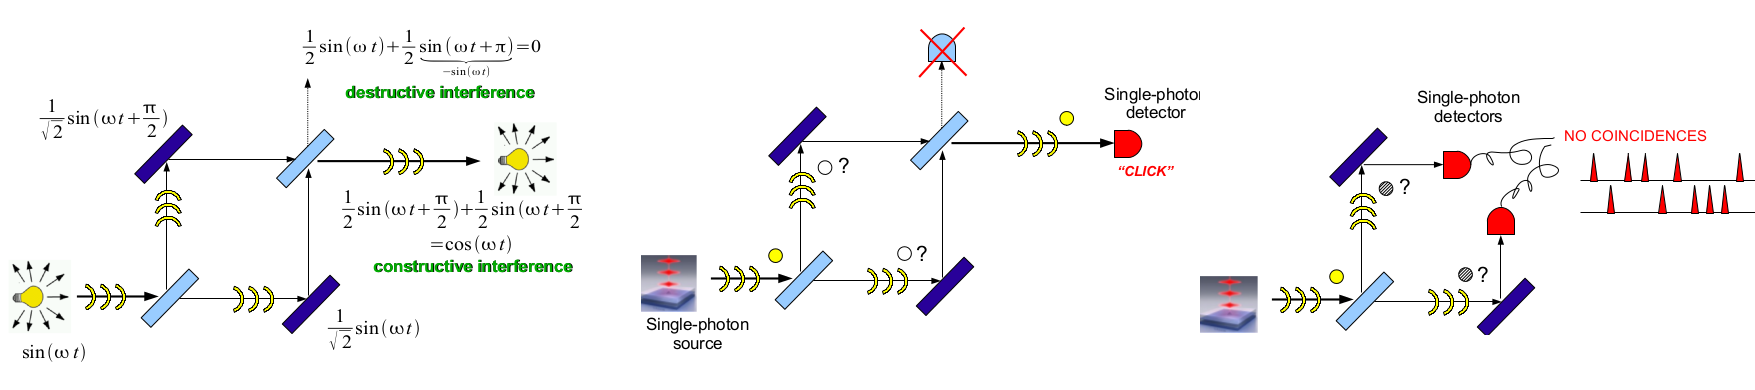
\includegraphics[scale=0.5]{ch1/image3.png}
	\captionof{figure}{ }
	\end{wrapfigure}
Il existe plusieurs sortes de section efficace. Pour s'en rendre compte, définissons ce
qu'est une collision. Il s'agit de \textit{l'interaction entre une particule incidente et une particule cible qui implique un effet spécifique mesurable}. Ainsi, la section efficace ne 
dépend pas que des particules incidentes/cibles et de leur vitesse \textbf{mais aussi} de l'effet
physique !\\
\ \\

Sur le grand nombre d'interaction existant, on peut s'intéresser à une perte d'énergie 
(section efficace différentielle en énergie $d\sigma/dE$) ou à une émission dans une 
direction donnée ((section efficace différentielle en énergie $d\sigma/d\Omega$).\\

	\begin{wrapfigure}[7]{r}{5cm}
	\vspace{-9mm}
	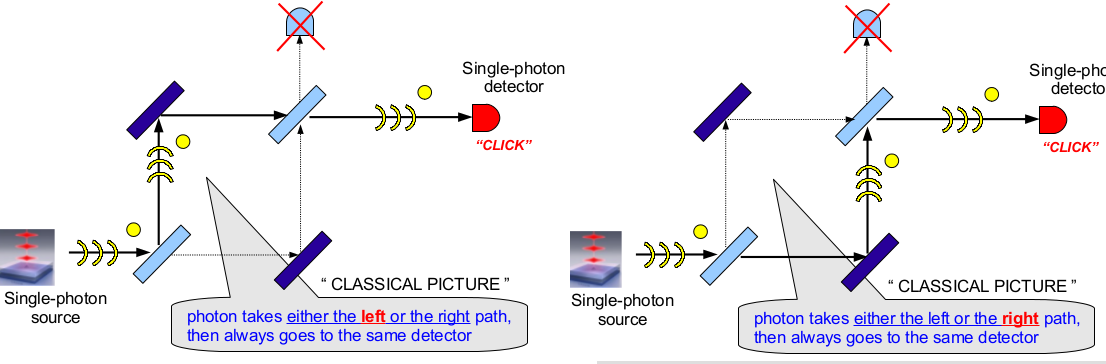
\includegraphics[scale=0.5]{ch1/image4.png}
	\captionof{figure}{ }
	\end{wrapfigure}
Quel est le rapport avec les valeurs moyennes annoncées ci-dessus ? Il n'est pas possible 
de déterminer expérimentalement les sections efficaces microscopiques en bombardant un 
atome avec une seule particule, il va falloir travailler avec des informations 
\textbf{statistiques} venant d'un bombardement (faisceau) sur la matière (milieu). Nous 
ferons l'hypothèse que les projectiles du faisceau n'interagissent pas entre-eux.\newpage

	\begin{wrapfigure}[9]{r}{4cm}
%	\vspace{-9mm}
	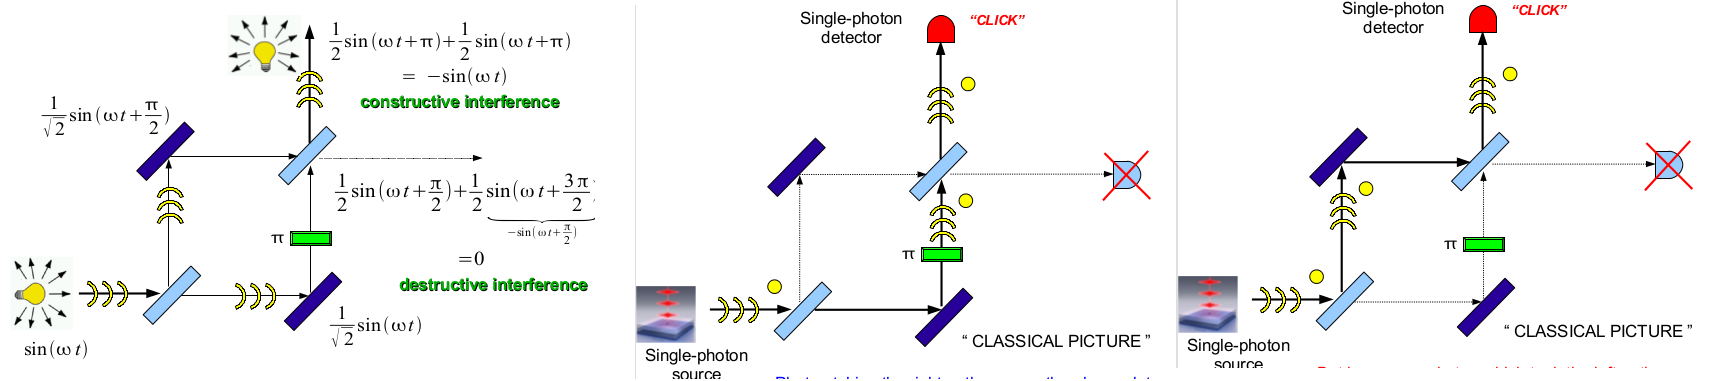
\includegraphics[scale=0.35]{ch1/image5.png}
	\captionof{figure}{ }
	\end{wrapfigure}
La section efficace sera ainsi définie par une probabilité. Soit un faisceau de particule
(densité de courant $J$), un milieu cible (aire $S$ plus petites que l'aire du faisceau)
et processus d'interaction $A$ (caractérisé par $\sigma_A$). Le nombre d'interaction $A$ 
induits par le faisceau par unité de temps $n_A$ s'écrit
\begin{equation}
n_A=JS\times\frac{\sigma_A}{S}=J\sigma_A
\end{equation}\ \\
Considérons un volume $V=S.x$ et une densité de particule cible $N$ 
\begin{equation}
n_A=N\times Sx\times J\sigma_A=JS\times Nx\sigma_A\quad\Rightarrow\quad P_A=Nx\sigma_A
 {\mbox{~~~~pour~~~~}}Nx\sigma_A\ll 1
\end{equation}
où $P_A$ est la probabilité pour un projectile de subir un processus $A$.\\

Dans le cas où $N.x.\sigma_A$ n'est pas petit, on peut observer une collision et, s'il 
n'y a pas d'absorption, la particule peut en subir une nouvelle : on parle de \textbf{
collisions multiples}. Soit $P_n$ la probabilité d'initier $n$ événements $A$. Cette 
situation est équivalente à considérer $n$ particules cibles dans un cylindre de volume 
$v=x.\sigma_A$ associé à une trajectoire. Ce problème est un classique de la théorie 
cinétique des gaz, on peut montrer que $P_n$ quit une distribution de Poisson
\begin{equation}
P_n=\frac{(Nv)^n}{n!}e^{-Nv}
\end{equation}
La valeur moyenne se définit alors comme
\begin{equation}
\langle n \rangle=Nv=Nx\sigma_A
\end{equation}
On en tire la \textsc{Loi de Lambert \& Beer} gouvernant les phénomènes d'absorption
\begin{equation}
P_0=e^{-Nx\sigma_A}
\end{equation}
Il s'agit de la probabilité de ne pas se faire absorbé. Si $Nx\sigma_A\ll 1$, on peut 
utiliser l'approximation suivante
\begin{equation}
P_n\simeq\left\{
\begin{aligned}
   &1-Nx\sigma_A& {\mbox{~~~~pour~~~~}} n=0\\
   &Nx\sigma_A& {\mbox{~~~~pour~~~~}} n=1\\
   &0&{\mbox{~~~~pour~~~~}} n\ge 2
\end{aligned} 
\right.
\end{equation}
Cette distribution nous permet de définir aisément la distance moyenne entre deux 
processus de type $A$, soit le \textbf{libre parcours moyen $\lambda_A$}
\begin{equation}
\lambda_A=\frac{1}{N\sigma_A}
\end{equation}
Ceci se généralise pour les processus multiples
\begin{equation}
\sigma_{total}=\sigma_A+\sigma_B+\sigma_C+\dots,\qquad \frac{1}{\lambda_{total}}=\frac{1}{\lambda_{A}}+\frac{1}{\lambda_{B}}+\frac{1}{\lambda_{C}}+\dots
\end{equation}


\subsubsection{Pouvoir d'arrêt}
Les pertes en énergies sont caractérisée par le \textbf{pouvoir d'arrêt} (\textit{stopping power}) : il s'agit de la grandeur la plus importante pour une particule chargée. Il s'agit - pour une 
particule chargée d'énergie cinétique $E$ dans un matériau - de la perte d'énergie moyenne
($\Delta E$) par unité de longueur subie par la particule le long de sa trajectoire ($\Delta x$)
\begin{equation}
\dfrac{\Delta E}{\Delta x}\qquad [J.M^{-1}] = [eV.m^{-1}]
\end{equation}
Afin de l'exprimer mathématiquement, considérons une cible de petite épaisseur (par rapport 
à la profondeur de pénétration) $\Delta x$ et un projectile d'énergie $E$. En considérant des 
pertes d'énergies discrète $T_j \ll E$ :
\begin{equation}
\Delta E = \sum_j n_jT_j
\end{equation}
L'énergie moyenne se calcule donc
\begin{equation}
\langle \Delta E \rangle= \sum_j \langle n_j \rangle T_j
\end{equation}
où $\langle n_j\rangle=N\Delta x\sigma_j$. Nous avons alors
\begin{equation}
\langle \Delta E \rangle = N \Delta x \sum_j T_j \sigma_j
\end{equation}
En définissant la \textbf{section efficace d'arrêt} $S$
\begin{equation}
S = \sum T_j\sigma_j
\end{equation}
On définit le \textbf{pouvoir d'arrêt}\ \\

\cadre{\begin{equation}
\frac{\langle \Delta E \rangle}{\Delta x}= NS=N\sum_j T_j \sigma_j
\end{equation}}\ \\

Le pouvoir d'arrêt est donc une propriété \textit{macroscopique} tandis que la section 
efficace d'arrêt est une propriété \textit{microscopique}.

\subsubsection{Paramètres de straggling}
Tant que nous sommes dans les statistiques, calculons les écarts quadratiques moyens des
fluctuations en énergie
\begin{equation}
\Omega^2=\overline{(\Delta E-\langle \Delta E \rangle)^2}
\end{equation}
En considérant $\Delta E-\langle \Delta E \rangle= \sum_j (n_j-\langle n_j \rangle) T_j$, 
on obtient
\begin{equation}
\overline{(\Delta E-\langle \Delta E \rangle)^2}= \sum_{j ,l}\overline{(n_j-\langle n_j \rangle) (n_l-\langle n_l \rangle)}T_jT_l
\end{equation}
Deux cas sont possibles
\begin{enumerate}
\item $j=l$; on peut utiliser les propriétés de la distribution de Poisson
\begin{equation}
\overline{(n_j-\langle n_j \rangle)^2}=\langle n_j \rangle=N\Delta x \sigma_j
\end{equation}
\item $j\neq m$; on transforme la moyenne du produit en produit des moyennes 
(ceci suggère l'indépendance statistiques des différents types de collisions)
\begin{equation}
\overline{(n_j-\langle n_j \rangle) (n_l-\langle n_l \rangle)}=\overline{(n_j-\langle n_j \rangle)}\times\overline{(n_l-\langle n_l \rangle)}
\end{equation}
Or, comme $\overline{n_j-\langle n_j \rangle}=0$, les termes avec $j\neq l$ sont nuls
\end{enumerate}
On obtient donc
\begin{equation}
\Omega^2=\sum_j\langle n_j \rangle T_j^2=N\Delta x\sum_jT_j^2\sigma_j=N\Delta xW
\end{equation}
où $W$ est le \textbf{paramètre de straggling} qui \textit{caractérise les fluctuations en 
énergie} et est défini comme\footnote{Paramètre microscopique.}\ \\

\cadre{\begin{equation}
W=\sum_j T_j^2 \sigma_j
\end{equation}}\ \\

\subsubsection{Notation intégrale et cible épaisse}
Comme annoncé, le grand nombre de collision implique une perte d'énergie quasi-continue (et 
donc un spectre continu)
\begin{equation}
\sigma_j \rightarrow \frac{d\sigma}{dT}\Delta T_j
\end{equation}
Si $\Delta T_j$ est suffisamment petit, les sommes deviennent des intégrales\ \\

\cadre{\begin{equation}
S = \int T\ d\sigma,\qquad\qquad\qquad W = \int T^2 d\sigma
\end{equation}
où $d\sigma =  \frac{d\sigma}{dT}dT$.}\ \\

Nous avions jusqu'ici considéré $\Delta x$ petit impliquant $E$ constant, mais en général $S$
et $W$ dépendent de $E$. En considérant que les fluctuations des pertes d'énergies sont 
négligeables, l'énergie $E$ est bien définie en fonction de la profondeur de pénétration 
$x$\footnote{$E\to E(x)$}. On fait alors l'\textit{approximation du ralentissement continu}
(\textit{Continuous Slowing Down Approximation} - CSDA)\ \\

\cadre{\begin{equation}
\dfrac{dE}{dx} = -NS(E)
\end{equation}
où le signe négatif tient compte de la diminution d'énergie du projectile.}\ \\

Le parcours (\textit{range}) $R$ d'une particule chargée d'énergie $E$ dans un milieu est 
la valeur moyenne $\langle l \rangle$ de la longueur $l$ de sa trajectoire suivie 
jusqu'à son arrêt (sans tenir compte du mouvement thermique). En CSDA, on trouve comme 
profondeur de pénétration
\begin{equation}
x=\int^{E}_{E(x)}\frac{dE'}{NS(E')}
\end{equation}
Le \textit{range} en CSDA est donné pour $x=l$ avec $E(l)=0$
\begin{equation}
R_{CSDA}=\int^{E}_{0}\frac{dE'}{NS(E')}
\end{equation}
Rappelons que cette expression valable pour un straggling en énergie négligeable, à cause 
de notre première hypothèse.


\subsubsection{Modèle classique du pouvoir d'arrêt}
Il s'agit d'un modèle classique non-relativiste établi en 1913 par Niels \textsc{Bohr} qui
est incroyablement correct pour une certaine plage d'énergie.\\

	\begin{wrapfigure}[7]{l}{7cm}
	\vspace{-8mm}
	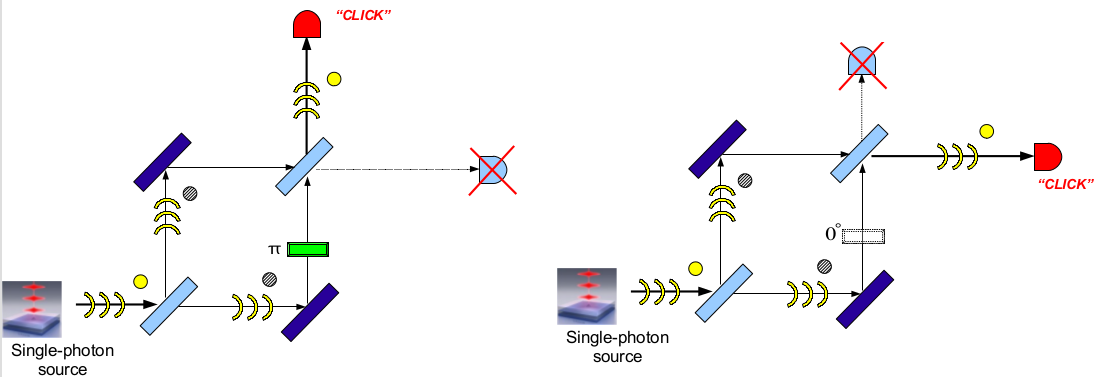
\includegraphics[scale=0.55]{ch1/image6.png}
	\captionof{figure}{ }
	\label{fig:1.6}
	\end{wrapfigure}
Soit un projectile de charge $e_1$, de masse $m_1$, de vitesse $v$ et une particule cible
($m_2,e_2$) initialement \textbf{au repos}. Cette condition initiale implique un 
\textit{scattering de Coulomb} avec un paramètre d'impact $p$\footnote{Pour rappel, il 
s'agit de la distance entre la trajectoire initiale de 1 et 2.} supposé \textit{pas trop 
petit} (\textit{soft collision}).\\

	\begin{wrapfigure}[9]{r}{6cm}
	\vspace{-8mm}
	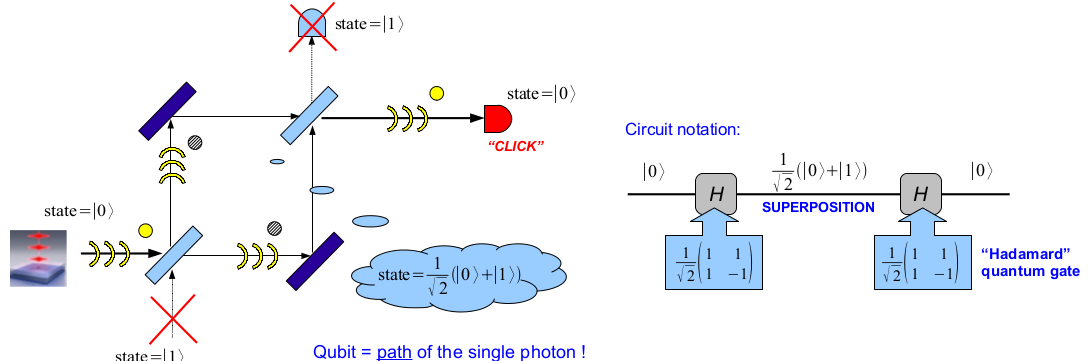
\includegraphics[scale=0.55]{ch1/image7.png}
	\captionof{figure}{ }
	\end{wrapfigure}
Supposons que la particule cible reçoit une quantité de mouvement faible tel qu'elle peut 
être considérée au repos durant l'interaction : on note le transfert de la quantité de
mouvement (unités CGS)
\begin{equation}
\overrightarrow{\Delta P}=\int_{-\infty}^{+\infty} dt \overrightarrow{F}(t)
\end{equation}
où $\DS F(t)=\frac{e_1e_2}{p^2+(vt)^2}$. En décomposant la force $\overrightarrow{F}=
F_{\parallel}\overrightarrow{1_{\parallel}}+F_{\perp}\overrightarrow{1_{\perp}}$, on 
obtient les composantes $\parallel$ et $\perp$ du transfert de quantité de mouvement\footnote{J'étais en retard\dots Quelqu'un à des notes? Sur le graphique surtout}
\begin{eqnarray}
&&\Delta P_\parallel=e_1e_2\int_{-\infty}^{+\infty}dt\frac{vt}{(p^2+(vt)^2)^{3/2}}=0\\
&&\Delta P_\perp=e_1e_2\int_{-\infty}^{+\infty}dt\frac{p}{(p^2+(vt)^2)^{3/2}}=\frac{2|e_1e_2|}{pv}
\end{eqnarray}
Il est possible d'estimer la durée de la collision, qui correspond au temps durant lequel 
le transfert d'énergie se passe
\begin{equation}
\Delta P_{\perp}\simeq F_{max}\tau
\end{equation}
où $F_{max} = e_1e_2/p^2$, la force pour la distance minimale d'approche ($p$ en $t=0$). En 
substituant, on trouve
\begin{equation}
\tau\simeq\frac{2p}{v} 
\end{equation}
Cette expression est cohérente avec la \autoref{fig:1.6} ($p/v$ à gauche et à droite, d'où le facteur 2).Il ne s'agit que d'un ordre de grandeur qui nous informe que les deux particules interagissent
de même façon effective sur une distance $2p$ le long de la trajectoire de la particule incidente.\\

	\begin{wrapfigure}[8]{l}{6cm}
	\vspace{-10mm}
	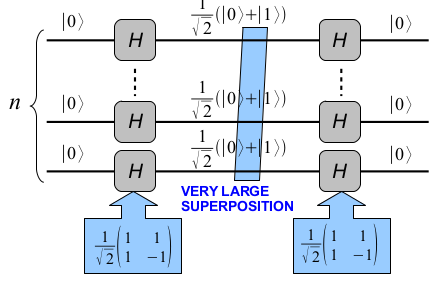
\includegraphics[scale=0.55]{ch1/image8.png}
	\captionof{figure}{ }
	\end{wrapfigure}
L'énergie $T$ transférée de 1 vers 2 s'obtient en explicitant $\Delta P_\perp^2$
\begin{equation}
T=\frac{\Delta P_\perp^2}{2m_2}\simeq \frac{2e_1^2e_2^2}{m_2v^2p^2}
\label{eq:1.ad}
\end{equation}
Le seul paramètre (aléatoire) dont dépend $T$ est le paramètre d'impact $p$. Ainsi, le nombre
de collisions caractérisés par un transfert d'énergie compris entre $T$ et $T+dT$ est caractérisé
par un paramètre d'impact entre $p$ et $p+dp$. Comme nous sommes en présence d'une géométrie
cylindrique, la particule incidente devra se trouver dans un anneau. La section efficace du 
projectile $d\sigma$ doit forcément être l'aire de cet anneau
\begin{equation}
d\sigma=2\pi pdp=\left|\frac{d(\pi p^2)}{dT}\right| dT
\label{eq:1.se}
\end{equation}
En calculant la dérivée de \eqref{eq:1.ad} dans l'expression \eqref{eq:1.se}, on trouve 
la forme de la section efficace de Rutherford pour la diffusion (scattering) coulombienne qui 
sera déduite bien plus tard (exactement) par la mécanique quantique.\ \\

\cadre{\begin{equation}
d\sigma \approx 2\pi\dfrac{e_1^2e_2^2}{m_2v^2}\dfrac{dT}{T^2}
\end{equation}}\ \\

\subsubsection{Résultats préliminaires}
Cette formule nous permet d'obtenir des résultats préliminaire pour le stopping et le 
straggling. Sachant que $S = \int Td\sigma$ et $W = \int T^2d\sigma$, on trouve
\begin{equation}
S\simeq 2\pi \frac{e_1^2e_2^2}{m_2v^2}\int_{T_{max}}^{T_{min}}\frac{dT}{T},\qquad\qquad
W\simeq 2\pi \frac{e_1^2e_2^2}{m_2v^2} \int_{T_{max}}^{T_{min}}dT
\end{equation}
Après intégration (à connaitre \textbf{par coeur}!)\ \\

\cadre{
\begin{eqnarray}
&&S\simeq 2\pi \frac{e_1^2e_2^2}{m_2v^2}\int_{T_{max}}^{T_{min}}\frac{dT}{T}\vspace{2mm}\\
&&W\simeq 2\pi \frac{e_1^2e_2^2}{m_2v^2} \int_{T_{max}}^{T_{min}}dT
\end{eqnarray}}\ \\

En utilisant le \textbf{nombre d'arrêt} (\textit{stopping number}) $\DS 
L=\frac{1}{2}\ln{\left(\frac{T_{max}}{T_{min}}\right)}$ on peut ré-écrire
\begin{equation}
S\simeq 4\pi \frac{e_1^2e_2^2}{m_2v^2}L
\end{equation}

\textsc{Résultats préliminaires pour le stopping}\ \\
Soit les électrons $(e)$ de la cible (densité $NZ_2$, masse $m$ et charge $-e$) et les 
noyaux $(n)$ de la cible (densité $N$, masse $M_2$ et charge $Z_2e$). On peut calculer 
l'énergie moyenne en multipliant $S_e$ par $NZ_2\Delta x$. En faisant de même pour $S_n$ :
\begin{eqnarray}
&&S_e=\frac{4\pi e_1^2e^2}{mv^2}L_e \Rightarrow  \langle \Delta E\rangle_e\simeq NZ_2\Delta x \times \frac{4\pi e_1^2e^2}{mv^2}L_e\vspace{2mm}\\
&&S_n=\frac{4\pi e_1^2Z_2^2e^2}{M_2v^2}L_n \Rightarrow  \langle \Delta E\rangle_n\simeq N\Delta x \times \frac{4\pi e_1^2Z_2^2e^2}{M_2v^2}L_n
\end{eqnarray}
Effectuons le rapport de ces deux dernières expressions
\begin{equation}
\frac{\langle \Delta E\rangle_n}{\langle \Delta E\rangle_e}\simeq \frac{m}{M_2}Z_2\frac{L_n}{L_e}
 {\mbox{~~or~~}} \frac{mZ_2}{M_2}<10^{-3}
\end{equation}
En laissant pour l'instant tomber le rapport des $L$ (straggling number), on obtient un terme 
inférieur à $10^{-3}$ : un électron incident va perdre beaucoup plus d'énergie lorsqu'il va 
interagir avec d'autres électrons plutôt qu'avec des neutrons.

\newpage
\subsubsection{Détermination de l'énergie transférée maximale $T_{max}$}
	\begin{wrapfigure}[8]{r}{3.5cm}
	\vspace{-5mm}
	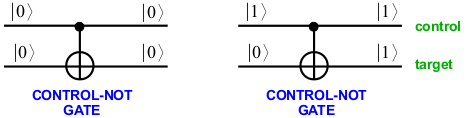
\includegraphics[scale=0.75]{ch1/image9.png}
	\captionof{figure}{ }
	\end{wrapfigure}
Soit $T_{max}$, l'énergie cinétique maximale qui peut être transférée dans une collision. 
Celle-ci est obtenue pour $p=0$, soit quand la particule cible est le plus proche possible
de la particule incidente. Nous ne sommes plus ici dans le cadre du précédent modèle (\textit{
soft collision}) mais ce n'est pas grave car seule une limite maximale est recherchée. L'image
ci-contre représente le système du laboratoire.\\

Dans le système du centre de masse (désigné par un \textit{prim})
\begin{equation}
v_{CM}=\frac{m_1v}{m_1+m_2},\qquad\qquad\qquad v'=v-v_{CM}
\end{equation}
Considérons une collision élastique avec uniquement un transfert d'énergie cinétique. L'intérêt
d'une telle collision dans le système du centre de masse est que seule la direction change : 
la vitesse et le module restent inchangés.
\begin{center}
	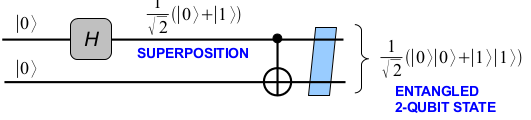
\includegraphics[scale=0.75]{ch1/image10.png}
	\captionof{figure}{ }
\end{center}
La situation correspondant à un maximum d'énergie transférée correspond à celle où la variation 
de la direction est la pus importante, soit quand tout change de sens. Dans le système du 
laboratoire, la vitesse maximale $v_{2,max}$ de la particule 2 s'écrit
\begin{equation}
v_{2,max}=\frac{2m_1v}{m_1+m_2}
\end{equation}
L'énergie maximale transférée vaut donc
\begin{equation}
T_{max}=\frac{m_2v_{2,max}^2}{2}=\gamma E
\end{equation}
où $\DS\gamma=\frac{4m_1m_2}{(m_1+m_2)^2} {\mbox{~~~~et~~~~}}E=\frac{m_1v^2}{2}$.\\

Ceci mène directement à deux implications 
\begin{enumerate}
\item Pour $m_1=m_2 \to \gamma=1$ ; l'énergie transférée peut valoir toute l'énergie de la particule
incidente
\item Pour $m_1\ll m_2$ ou l'inverse $\to \gamma$ petit
\end{enumerate}
Il en vient que\\

\cadre{\begin{itemize}
\item[$\bullet$] Un grand transfert d'énergie est possible pour l'interaction $e^-/e^-$
\item[$\bullet$] Un petit transfert d'énergie est possible pour l'interaction ion$/e^-$
\item[$\bullet$] Un petit transfert d'énergie est possible pour l'interaction $e^-/$ion
\item[$\bullet$] Un petit transfert d'énergie est possible pour l'interaction ion/ion
\end{itemize}
Notons que l'on parle de transfert possible et \textbf{pas} de probabilité.}

\newpage
\subsubsection{Détermination de l'énergie transférée minimale $T_{min}$}
Nous allons calculer $T_{min}$ dans le cas d'une collision avec un $e^-$ (il s'agit du cas
pratique le plus intéressant). Pour un électron isolé et libre, on trouve $T_{min}=0$. Or, 
la section efficace de stopping contient le logarithme du rapport $T_{max}/T_{min}$, il y 
aura divergence. Deux façon de lever la divergence existent
\begin{enumerate}
\item Considérer que les $e^-$ sont liés à une molécule ou à un atome
\item Considérer l'écrantage de l'interaction de Coulomb
\end{enumerate}
La première solution sera retenue?. Le plus simple est le modèle simple de Thompson où 
$T_{min}$ est l'énergie d'excitation la plus faible. Néanmoins, on s'intéressera ici 
au modèle de Bohr, plus proche du résultat quantique.\\

La vision de Bohr revient à voir la matière comme une collection d'oscillateurs harmonique 
classiques. En cas de choc lent $(2\pi/\omega_0\ll \tau$), l'oscillateur peut directement 
se remettre en place et le transfert d'énergie est négligeable (invariance adiabatique). 
L'orbite de l'électron n'est que provisoirement déformée, les états initiaux et finaux sont
identiques.\\

Si par contre le temps d'interaction est court par rapport à la période de l'oscillateur 
($\tau \ll 2\pi/\omega_0$), l'oscillateur reçoit une impulsion $F\times\tau$. C'est ce que
nous considérons ici. En utilisant l'expression du temps d'interaction, on trouve un ordre
pour $T_{min}$
\begin{equation}
\frac{2p}{v}\ll\frac{2\pi}{\omega_0} \Rightarrow p_{max}\sim\frac{v}{\omega_0}
 \Rightarrow T_{min}\sim\frac{2e_1^2e^2\omega_0^2}{mv^4}
\end{equation}
avec $\DS T\simeq \frac{2e_1^2e_2^2}{mv^2p^2}$ et $p_{max}$, le 
\textit{rayon adiabatique de Bohr}.\\

On peut alors, dans le modèle de Bohr (en reprenant les précedentes expressions), calculer 
la section efficace de stopping électronique comme il n'y a plus divergence \\

\cadre{\begin{equation}
S_e=\frac{4\pi Z_2 e_1^2e^2}{mv^2}L_e\quad\text{avec}\quad L_e=\ln\frac{Cmv^3}{|e_1e
|\omega_0}{\mbox{~~et~~}}C\simeq 1
\end{equation}
où $L=\frac{1}{2}\ln{\left(\frac{T_{max}}{T_{min}}\right)}$ et $C$, une correction introduite 
par Bohr que nous ne prendrons pas en compte.}


\subsubsection{Déviation angulaire maximale}
Soit $m_2\leq m_1$. Soit à gauche le référentiel du laboratoire et à droite, celui du centre de 
masse
\begin{center}
	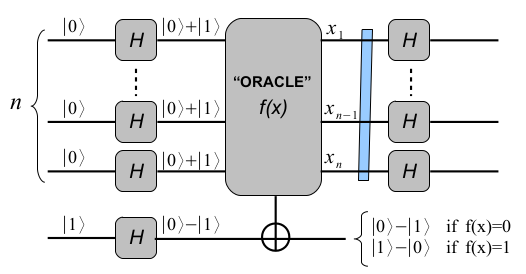
\includegraphics[scale=0.45]{ch1/image11.png}
	\captionof{figure}{ }
\end{center}
Dans le référentiel du centre de masse
\begin{equation}
v_{CM}=\frac{m_1}{m_1+m_2}v_{1i},\qquad\qquad\qquad v'=v-v_{CM}
\end{equation}
On en tire
\begin{equation}
v'_{1i}=v_{1i}-v_{CM}=\frac{m_2}{m_1+m_2}v_{1i}
\end{equation}
Comme nous avons une collision élastique dans le repère du centre de masse, seule la direction
est modifiée (et donc $v_{1f}'=v_{1i}'$)
\begin{equation}
v'_{1f}=\frac{m_2}{m_1+m_2}v_{1i}
\end{equation}

	\begin{wrapfigure}[8]{r}{5.5cm}
	\vspace{-5mm}
	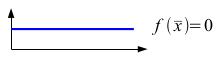
\includegraphics[scale=0.65]{ch1/image12.png}
	\captionof{figure}{ }
	\end{wrapfigure}

L'angle maximal $\theta_{max}$ est obtenu lorsqu'un angle droit est formé au niveau de la
circonférence du cercle. On choisit alors $v_{1f}'$ ($v_{CM}$) étant fixé de sorte à avoir
$\theta_{max}$. Après un peu de trigonométrie
\begin{equation}
\sin{\theta_{max}}=\frac{v'_{1f}}{v_{CM}}=\frac{m_2}{m_1}
\end{equation}
Si $m_2\geq m_1$, on trouve $\theta_{max}=\pi$. \\

En conclusion\\

\cadre{\begin{itemize}
\item[$\bullet$] Grandes déviations possibles ($\theta_{max}=\pi/2$) pour l'interaction $e^-/e^-$
\item[$\bullet$] Très grandes déviations possibles ($\theta_{max}=\pi$) pour l'interaction $e^-/$ion
\item[$\bullet$] Petites déviations pour l'interaction ion/$e^-$
\item[$\bullet$] Grandes déviations possibles (dépendant de $m_1$ et $m_2$) pour l'interaction ion/
ion
\end{itemize}}

\subsection{Conclusions à propos de ces considérations de base}
\subsubsection{Pour les ions incidents}
De façon générale les pertes électroniques dominent (petits transfert d'énergie et petites déviations
angulaires) et les pertes nucléaires (collisions noyaux) sont rares (se produisent pour un 
faible nombre de projectives mais de grand transferts d'énergies sont possibles ainsi que de 
grandes déviations angulaires). Ils ont une \textit{trajectoire rectilignes accompagnées de 
pertes d'énergie faibles et continues}.

\subsubsection{Pour les électrons incidents}
Les pertes électroniques dominent (mais cette fois grands transferts d'énergie et grandes déviations
angulaires possibles). On retrouve aussi des pertes nucléaires (petits transferts d'énergie mais
très grandes déviations angulaires possibles (possibilité de rétro-diffusion). Ils ont une 
\textit{trajectoire courbée accompagnée de grandes pertes d'énergie}.






\chapter{Interaction des ions avec la matière}
	\begin{wrapfigure}[11]{l}{10.5cm}
	\vspace{-5mm}
	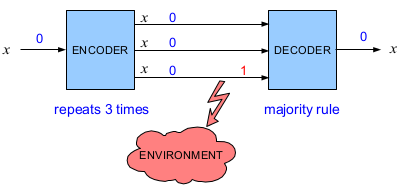
\includegraphics[scale=0.3]{ch2/image1.png}
	\captionof{figure}{ }
	\end{wrapfigure}
Ci-contre, à gauche, sont représenté les trajectoires de particules $\alpha$ d'une énergie
de 5.5 MeV. On observe que trois d'entre-elles sont rentrées en collisions avec les noyaux
(déviation angulaire plus importante). A droite, considérons un proton incident sur 
de l'aluminium, décrit par le modèle de Bohr. Ce modèle étant classique, il ne peut pas être
correct dans la zone relativiste. Lorsque la vitesse du projectile se rapproche de $v_0$, 
la vitesse de Bohr\footnote{On associe l'énergie à une certaine vitesse via l'énergie cinétique.}, 
on ne peut plus considérer que la particule est au repos, le modèle n'est dès lors plus 
valable\footnote{L'hypothèse de Bohr est telle que la particule cible est au repos.}

\section{Modèle semi-classique du pouvoir d'arrêt électronique}
Un rappel sur les oscillateurs classiques et l'approximation dipolaire est faite dans les
slides 5 à 12 : n'étant que des rappels/pré-requis, ils ne sont pas repris ici.

\subsection{Vitesses intermédiaires : $v_0\ll v \ll c$}
Dans le modèle semi-classique de \textsc{Bethe} (\textit{1930}), le noyau est traité 
classiquement et les électrons quantiquement, ils ne sont plus traités comme des oscillateurs
classiques. On s'intéresse ici au cas ou le modèle de Borh est correct. \\

Considérons un atome cible avec $Z_2$ électrons (masse $m$) et les états stationnaires $\ket j$ 
d'énergie $\epsilon_j$ où $j$ est un nombre quantique tel que $j=0$ dénote l'état fondamental. 
Les fréquences de résonance pour un atome dans son état initial sont données par
\begin{equation}
\hbar\omega_{j0}=\epsilon_j-\epsilon_0
\end{equation}
On dira que les électrons sont au repos durant l'interaction si $v\gg v_0$.
\\

Pour une énergie $Q$ perdue par l'ion incident, \textsc{Bethe} a posé
\begin{equation}
S=\sum_j\int Q d\sigma_Rf_{j0}(Q)
\end{equation}
où $\sigma_R$ est la section efficace de \textsc{Coulomb} pour un transfert d'énergie $Q$ 
(où $R$ pour \textsc{Rutherford}) et $f_{j0}$ sont les \textit{forces d'oscillateur généralisées}
qui incluent tous les effets quantiques pour la section efficace d'arrêt : ils décrivent les 
probabilités de transition entre les états pour une énergie transférée $Q$ donnée.\\

Afin de déterminer l'expression de $f_{j0}$, résolvons l'équation de Schrödinger dépendante du 
temps (celle-ci gouverne le mouvement électronique)
\begin{equation}
(H+V)\Psi(\overrightarrow{r},t)=i\hbar \frac{d\Psi(\overrightarrow{r},t)}{dt}
\end{equation}
où $H$ est l'hamiltonien d'un atome isolé de la cible, $\Psi(t)$ la fonction d'onde d'un état
lié et $V$ le potentiel décrivant l'interaction avec le projectile donné par
\begin{equation}
V(\overrightarrow{r},t)=\sum_{\nu=1}^{Z_2}\frac{-e_1e}{\overrightarrow{r}_\nu-\overrightarrow{R}(t)}
\end{equation}
où $\vec r = (\vec{r}_1,\dots \vec{r}_{Z_2})$ représente la trajectoire du projectile avec 
$\vec r_\nu$ l'opérateur position du $\nu^e$  électron et $\vec{R}=\vec{p}+\vec{v}t$. Développons
$\Psi(t)$ sur la base formée des états stationnaires
\begin{equation}
\Psi(\overrightarrow{r},t)=\sum_{j}c_j(t)e^{-i\epsilon_jt}|j\rangle
\end{equation}
où $\ket j$ sont les solutions de $H\ket j = \epsilon_j\ket j$. Dans le cadre de la méthode des
perturbations au premier ordre, on peut développer les coefficients $c_j$ en puissance du 
potentiel perturbatif $V$
\begin{equation}
c_j(t) = \delta_{j0} + c^{(1)}_j(t) + c^{(2)}_j(t) + \dots
\end{equation}
avec $\delta$ le symbole de Kronecker et

\begin{eqnarray}
c_j^{(1)}(t)=\frac{1}{i\hbar}\int_{-\infty}^{t}dt'e^{i\omega_{j0}t'}\langle j|V(\overrightarrow{r},t')|0\rangle\\
c_j^{(2)}(t)= \left(\frac{1}{i\hbar}\right)^2\sum_k\int_{-\infty}^{t}dt'e^{i\omega_{jk}t'}\langle j|V(\overrightarrow{r},t')|k\rangle
\times \int_{-\infty}^{t'}dt''e^{i\omega_{k0}t''}\langle k|V(\overrightarrow{r},t'')|0\rangle
\end{eqnarray}
et ainsi de suite mais ici nous ne nous intéressons que aux coefficients $c_j^{(1)}(\infty)$ car
seul le premier ordre nous intéresses. Ceux-ci représentent les amplitudes de transition. 
Substituons $c_j^{(1)}(\infty)$ dans l'expression explicite du potentiel, prenons-en la 
transformée de \textsc{Fourier} et intégrons sur $t'$
\begin{equation}
c_j^{(1)}(\infty)=\frac{-e_1e}{i\pi\hbar}\int \overrightarrow{dq}\frac{e^{-i\overrightarrow{q}.\overrightarrow{p}}}{q^2}F_{j0}(\overrightarrow{q})\delta(\omega_{j0}-\overrightarrow{q}.\overrightarrow{v})
\end{equation}
où $\DS F_{j0}(\overrightarrow{q})=\left\langle j\left| \sum_{\nu=1}^{Z_2}e^{i\overrightarrow{q}.\overrightarrow{r_\nu}}\right| 0\right\rangle$. Notons $Q=\frac{\hbar^2q^2}{2m}$. Par le 
\textsc{Postulat IV} de la mécanique quantique, les probabilités de transitions sont données 
par
\begin{equation}
P_j(p)=\left| \langle j| \Psi(\infty)\rangle\right|^2
\end{equation}
Ce qui donne dans le cadre de la méthode des perturbations au premier ordre
\begin{equation}
P_j(p)=\left| c_j^{(1)}(\infty)\right|^2
\end{equation}
Pour que $c_j^{(1)}(\infty) \neq 0$ pour $\omega_{j0} < q\nu$, il faut que (condition sur $Q$)
\begin{equation}
\omega_{j0}^2<q^2v^2 \Rightarrow 2mv^2Q>(\epsilon_j-\epsilon_0)^2
\end{equation}

\subsubsection{Approximation des collisions distantes - Approximation dipolaire}
Afin d'obtenir notre expression de $f_{j0}$, nous allons devoir utiliser une approximation. 
Considérons $c_j^{(1)}(\infty)$ à grand $p$ (\textit{collisions distantes}). Par l'approximation
dipolaire
\begin{equation}
e^{i\overrightarrow{q}.\overrightarrow{r}}\simeq 1+i\overrightarrow{q}.\overrightarrow{r}
\end{equation}
On obtient donc
\begin{equation}
F_{j0}(\overrightarrow{q})\simeq i\overrightarrow{q}\left\langle j\left| \sum_{\nu=1}^{Z_2}\overrightarrow{r_\nu}\right| 0\right\rangle
\end{equation}
En choisissant l'axe $x$ selon la vitesse du projectile et l'axe $y$ selon le paramètre 
d'impact, on voit apparaître des fonctions de \textsc{Bessel} modifiée $K_{0,1}$, d'ordre 0 et 1
\begin{equation}
c_j^{(1)}(\infty)=-\frac{2e_1e\omega_{j0}}{i\hbar v^2}\left\langle j\left| \sum_{\nu}^{Z_2}\overrightarrow{r}_\nu \right|0\right\rangle
 \times\left(iK_0\left(\frac{\omega_{j0}p}{v}\right),K_1\left(\frac{\omega_{j0}p}{v}\right),0\right)
\end{equation}
Les probabilités de transitions deviennent donc (données par $|c_j|^2$)
\begin{equation}
P_j(p)=-\frac{2e_1^2e^2Z_2}{mv^2p^2\hbar\omega_{j0}}f_{j0}
 \times\left\{\left[\frac{\omega_{j0}p}{v}K_0\left(\frac{\omega_{j0}p}{v}\right)\right]^2+\left[\frac{\omega_{j0}p}{v}K_1\left(\frac{\omega_{j0}p}{v}\right)\right]^2\right\}
\end{equation}
La grandeur $f_{j0}$ est appelée la \textbf{force d'oscillateur dipolaire} et a comme
expression
\begin{equation}
f_{j0}=\frac{2m}{3\hbar^2Z_2}(\epsilon_j-\epsilon_0)\left|\left\langle j\left|\sum_{\nu}^{Z_2}\overrightarrow{r}_\nu\right|0\right\rangle\right|^2
\end{equation}
Avec la règle de somme de \textsc{Thomas-Reiche-Kuhn} $\sum_j f_{j0}=1$.

\subsubsection{Comparaison modèle classique et semi-classique}
Maintenant que nous avons la probabilité d'une transition, il nous faut l'énergie moyenne. 
Considérons l'énergie transférée moyenne $T_{moy}$
\begin{equation}
T_{moy}(p)=\sum_jP_j(p)\hbar\omega_{j0}
\end{equation}
Comparons cette expression avec le résultat classique donné par 
\begin{equation}
T= \frac{2e_1^2e^2}{mv^2p^2}f_{dist}(p),\qquad\text{ où }\quad 
f_{dist}(p)=\left[\frac{\omega_{0}p}{v}K_0\left(\frac{\omega_{0}p}{v}\right)\right]^2+\left[\frac{\omega_{0}p}{v}K_1\left(\frac{\omega_{0}p}{v}\right)\right]^2
\end{equation}
Les expressions sont identiques à condition que
\begin{equation}
f_{dist}(p)=\sum_jf_{j0}\left[\frac{\omega_{j0}p}{v}K_0\left(\frac{\omega_{j0}p}{v}\right)\right]^2+\left[\frac{\omega_{j0}p}{v}K_1\left(\frac{\omega_{j0}p}{v}\right)\right]^2
\end{equation}
Pour généraliser les fonctions $f_{j0}$ que nous venons d'élaborer aux grandes valeurs de $Q$, 
\textsc{Bethe} a posé
\begin{equation}
f_{j0}(Q)=\frac{1}{Z_2}\frac{\epsilon_j-\epsilon_0}{Q}|F_{j0}(\overrightarrow{q})|^2
\end{equation}
Avec cette forme la, lorsque $Q$ est petit, on retrouve l'expression que nous venons de calculer
\begin{equation}
f_{j0}(Q)\big\vert_{Q\simeq 0}=f_{j0}
\end{equation}

\subsubsection{Pouvoir d'arrêt : formule de Bethe}
Il est nécessaire de faire la distinction entre les collisions distantes ou proche (via $p$), soit 
les collision avec une grande ou petite quantité de mouvement transférée (via $q$) ou encore 
les collisions avec une grande ou petite énergie transférée (via $Q$). Pour se faire, 
nous allons séparer l'intégrale suivante en deux parties par rapport à $Q_0$
\begin{equation}
S=\sum_j\int Q d\sigma_Rf_{j0}(Q)
\end{equation}
$\bullet$ Pour $Q<Q_0$, l'approximation dipolaire est valide ($Q_0$)
\begin{equation}
S_{dist}=\sum_jf_{j0}\int_{(\epsilon_j-\epsilon_0)^2/2mv^2}^{Q_0} Q d\sigma_R
\end{equation}

$\bullet$ Pour $Q>Q_0$, il faut déterminer la borne supérieure de l'intégrale. On considère que 
la masse d'un ion $m_1\gg m$, la masse d'un électron.
\begin{equation}
T_{max} = \gamma E = \frac{4m_1m}{(m_1+m)^2}\frac{m_v^2}{2} \approx 2mv^2
\end{equation}
où nous avons négliger $m$ par rapport à $m_1$. On trouve alors la section efficace 
d'arrêt suivante
\begin{equation}
S_{proche}=\int_{Q_0}^{2mv^2} Q d\sigma_R\sum_jf_{j0}(Q)
\end{equation}
\textsc{Bethe} a démontré que
\begin{equation}
\sum_jf_{j0}(Q)=1
\end{equation}
Nous avons alors
\begin{equation}
S_{proche}=\int_{Q_0}^{2mv^2} Q d\sigma_R\equiv \sum_jf_{j0}\int_{Q_0}^{2mv^2} Q d\sigma_R
\end{equation}
En sommant les collisions proches et distantes, on trouve finalement
\begin{equation}
S=S_{proche}+S_{dist}= \sum_jf_{j0}\int_{(\epsilon_j-\epsilon_0)/2mv^2}^{2mv^2} Q d\sigma_R
\end{equation}
En considérant l'expression explicite $d\sigma_R= 2\pi \frac{e_1^2e_2^2}{m_2v^2}\frac{dQ}{Q^2}$, 
on obtient
\begin{equation}
S=\frac{4\pi e_1^2e^2}{mv^2}Z_2\sum_jf_{j0}\ln{\frac{2mv^2}{\epsilon_j-\epsilon_0}}
\end{equation}
La formule du pouvoir d'arrêt de \textsc{Bethe} se note généralement\\

\cadre{\begin{equation}
S_{e}=\frac{4\pi e_1^2e^2}{mv^2}Z_2\ln{\frac{2mv^2}{I}}
\end{equation}
où $I$ est définie comme l'énergie moyenne d'excitation telle que $\ln I=\sum_j f_{j0}\ln{
(\epsilon_j-\epsilon_0)}$. Ceci n'est valable que \textbf{si} $m_1\gg m, v\gg v_0 \to mv^2 \gg
 \hbar \omega_0$.}\ \\
 
On peut facilement comparer le modèle de \textsc{Bethe} à celui de \textsc{Bohr} via 
\begin{equation}
S_e=\frac{4\pi Z_2 e_1^2e^2}{mv^2}L_e
\end{equation}
où 
\begin{equation}
L_e=\ln\frac{Cmv^3}{|e_1e|\omega_0}
\end{equation}
pour le \textsc{Bohr} et 
\begin{equation}
L_e=\ln{\frac{2mv^2}{I}}
\end{equation}
pour \textsc{Bethe}.

\subsubsection{Dépendances principales du pouvoir d'arrêt}
Le pouvoir d'arrêt se compose lui-même de trois dépendances\ \\

\retenir{\begin{equation}
-\left( \frac{dE}{dx}\right)_{elec}=NS_{e}=\frac{4\pi e_1^2e^2}{mv^2}NZ_2\ln{\frac{2mv^2}{I}}
\end{equation}}\ \\

Les dépendances sont les suivantes
\begin{enumerate}
\item $\frac{4\pi e_1^2e^2}{mv^2}\Rightarrow{\mbox{D\'ependance principale dans la vitesse}}$, plus la vitesse augmente, plus le pouvoir d'arrêt diminue.
\item $NZ_2\Rightarrow{\mbox{D\'ependance principale dans le mat\'eriau}}$, plus il est grand, plus le pouvoir augmente.
\item $\ln{\frac{2mv^2}{I}}\Rightarrow{\mbox{D\'ependance faible dans la vitesse et dans le mat\'eriau}}$
\end{enumerate}

	\subsubsection{Énergies moyenne d'excitation}
	\begin{wrapfigure}[7]{r}{6.5cm}
	\vspace{-5mm}
	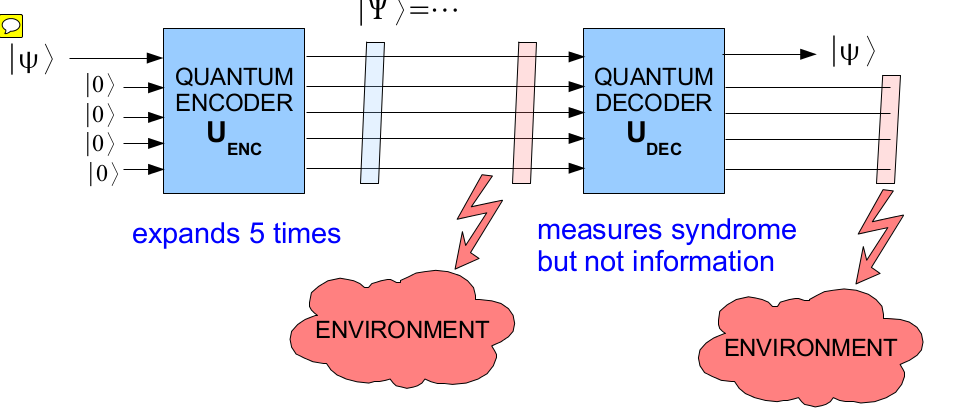
\includegraphics[scale=0.5]{ch2/image2.png}
	\captionof{figure}{ }
	\end{wrapfigure}
	

L'énergie moyenne d'excitation $I$ ne dépend \textbf{que} du matériau et \textbf{pas} du 
projectile. Il est possible de le calculer mais tout le monde s'en fiche car on peut l'obtenir
expérimentalement\footnote{De plus, comme il intervient dans $\log S$ il n'est pas nécessaire
de connaître sa valeur avec précision} via des formules empiriques. Celui-ci varie approximativement
linéairement (les irrégularités sont dues à la structure en couches de l'atome) avec $Z$ :
\textit{modèle de l'atome de Thomas-Fermi} où les électrons atomiques forment un gaz.

\newpage
\subsection{Grandes vitesses - Équation de \textsc{Bethe-Bloch} : $v_0<v\approx c$}
\textsc{Bloch} a apporté de nombreuses corrections à l'équation de \textsc{Bethe} pour 
former l'équation de \textsc{Bethe-Block}\\

\cadre{\begin{equation}
S_e = \dfrac{4\pi r_e^2mc^2}{\beta^2}Zz^2L(\beta)
\end{equation}
où $\DS L(\beta)= L_0(\beta) = \frac{1}{2}\ln\left(\frac{2mc^2\beta^2W_m}{1-\beta^2}\right)
-\beta^2-\ln I-\frac{C}{Z}-\frac{\delta}{2}$.}\ \\

Il s'agit en réalité de la même équation mais notée différemment, toute la différence se 
trouve dans le \textit{stopping number} $L$ qui contient donc les termes correctifs. 
Intéressons-nous à ceux-ci
\begin{itemize}
\item[$\bullet$] \textit{Corrections dues aux collisions}\ \\
$W_m$ donne l'énergie maximale transférée en une collision à un électron
libre\footnote{Il s'agit d'une expression relativiste non-approchée}
\begin{equation}
W_m=\frac{2mc^2\beta^2}{1-\beta^2}\left[1+\frac{2m}{m_1(1-\beta^2)^{1/2}}+\left(\frac{m}{m_1}\right)^2\right]^{-1}
\end{equation}
Pour $m_1\gg m$, on retrouve bien $2m\gamma_1^2v^2$.
\item[$\bullet$] \textit{Corrections relativistes}\ \\
Si $v\approx c$, il faut apporter des corrections relativistes. Lorsque l'on travaille avec
des vitesses relativistes, il faut considérer des électrons de plus en plus lointain ce qui, 
forcément, augmente le pouvoir d'arrêt. En effet, $p_{max} \propto \gamma_1v/\omega_0$ ce qui
montre que le paramètre d'impact augmente lorsque la vitesse fait de même. Le calcul relativiste
classique du champ donne
\begin{equation}
\overrightarrow{E}(\omega)=-\frac{e_1\omega}{\pi \gamma_1v^2}\left(\frac{i}{\gamma_1}K_0\left(\frac{\omega_{j0}p}{\gamma_1v}\right),K_1\left(\frac{\omega_{j0}p}{\gamma_1v}\right),0\right)
\end{equation}
On y voit apparaître des $\gamma_1$ et $f(p)$ se voit modifiée par ce fameux terme
\begin{equation}
f_{dist}(p)=\frac{1}{\gamma_1^2}\left[\frac{\omega_{0}p}{\gamma_1v}K_0\left(\frac{\omega_{0}p}{\gamma_1v}\right)\right]^2+\left[\frac{\omega_{0}p}{\gamma_1v}K_1\left(\frac{\omega_{0}p}{\gamma_1v}\right)\right]^2
\end{equation}
La composante principale en la vitesse se voit modifiée
\begin{equation}
\frac{4\pi e_1^2e^2}{mv^2}\Rightarrow \frac{4\pi e_1^2e^2}{m\gamma_1^2v^2}=\frac{4\pi e_1^2e^2}{mv^2}(1-\beta^2)
\end{equation}
où le $(1-\beta^2)$ apparaissant permet de comprendre le terme correspondant dans la formule de 
\textsc{Bethe-Bloch}, il va être possible de lui donner un sens physique. Sachant que la quantité 
de mouvement de la particule incidente devient $m\gamma_1v$, on en tire
\begin{equation}
T_{max}=2m\gamma_1^2v^2
\end{equation}
La composant logarithmique se modifie selon
\begin{equation}
\ln{\frac{2mv^2}{I}}\Rightarrow \ln{\frac{2m\gamma_1^2v^2}{I}}=\ln{\frac{2mv^2}{I(1-\beta^2)}}
\end{equation}
La combinaison de toutes ces relations implique donc que le pouvoir d'arrêt augmente lorsque 
la vitesse augmente, ce qui est la conséquence du traitement relativiste. 
\end{itemize}

\newpage

\begin{itemize}
\item[$\bullet$] \textit{Correction de densité}\ \\
Le terme correspondant à ces corrections est le $-\delta/2$. La formule de \textsc{Bethe} est 
valable pour un gaz de faible densité (atomes isolés) mais pour un solide il faut tenir compte
des effets collectifs d'un grand nombres d'atomes : on peut utiliser le modèle de Fermi. Une 
particule chargée incidente va polariser le milieu. Le champ électrique induit va alors donner un
moment dipolaire électrique aux atomes et il en résultera un champ électrique opposé à celui 
produit par la particule chargée. Le champ électrique sera donc réduit via l'écrantage des dipôles.\\

A cause de cette diminution du champ (à cause de la polarisation), les atomes lointains ont un 
effet plus faible. L'effet de densité apparaît surtout aux grandes vitesses, en même temps que les 
effets relativiste (ils vont se "compenser"). S'il n'est signifiant qu'aux énergies élevées c'est 
à cause du facteur $\gamma_1$ présent dans $p_{max}$ qui augmente l'erreur commise en ignorant la
polarisation du milieu : si $v$ augmente, $p_{max}$ augmente et donc $\delta/2$ augmente causant une
diminution de $S$.

\begin{center}
	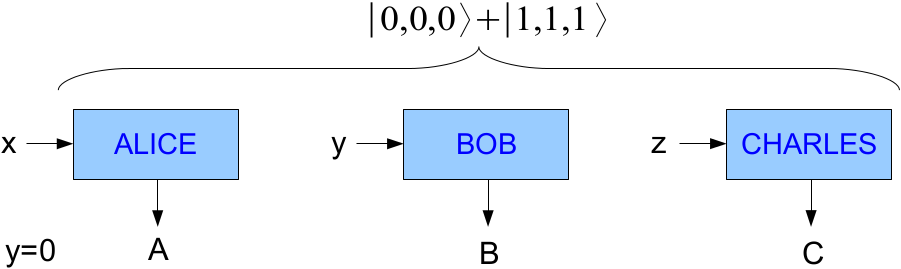
\includegraphics[scale=0.5]{ch2/image3.png}
	\captionof{figure}{L'effet relativiste et de densité vont se stabiliser de sorte que le 
	pouvoir d'arrêt devient constant. On parle alors de \textit{plateau de Fermi}, constant à
	grande vitesse.}
\end{center}

On peut écrire la correction de densité
\begin{equation}
\frac{\delta}{2}=\ln{\frac{\hbar\omega_p}{I}}+\ln{\gamma_1\beta}-\frac{1}{2}
\end{equation}
avec $\omega_p=\sqrt\frac{ne^2}{\epsilon_0m}$ la \textit{pulsation plasma}, mais ceci est plus
informatif.

\item[$\bullet$] \textit{Correction shell} ("en couches")\ \\
Il s'agit du terme $-C/Z$. Nos deux formules sont basées sur l'hypothèse que $v\gg v_0$ (permet
de calculer $I$ moyen). Lorsque que n'est plus le cas, on ne peut plus considérer que tous les
électrons ont la même énergie de liaison. Le problème est que certains électrons sont plus liés 
que d'autres. Comme ils seront plus durs à arracher, leur contribution au pouvoir d'arrêt va 
diminuer et il ne faudra plus les considérer. On ajoute ainsi un terme de correction "moyen" qui
réduit $S$ de maximum 6\% qui ne dépend que de la vitesse et du matériau considéré, peu importe 
les couches. Il existe deux méthodes pour calculer $C/Z$
	\begin{enumerate}
	\item Une basées sur les fonctions d'ondes hydrogénoïdes (HWF)\footnote{Un électron interne ne
	 peut
	 pas être représenté par une fonction d'onde de la sorte mais comme la rigueur absolue n'est 
	 pas possible en s'en contentera car \textit{au moins} on a un résultat, bien que moins 
	 rigoureux.}
	\item Une basée sur l'approximation en densité locale (LDA)
	\end{enumerate}
	
%\begin{center}
\hspace{-1cm}	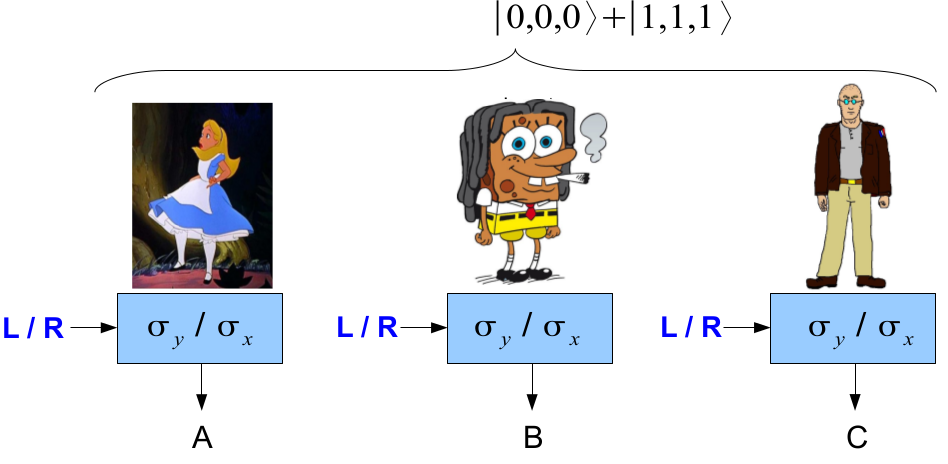
\includegraphics[scale=0.4]{ch2/image4.png}
	\captionof{figure}{A gauche la comparaison théorie/expérience (relativement bonne et comme la
	correction est logarithmique on s'en contentera), au centre le calcul par la méthode LDA et à
	droite selon HWF. L'écart entre les méthodes est plus grand pour des $Z$ élevés mais 
	les deux sont globalement assez bonnes.}
%\end{center}
\end{itemize} \ \\

Il est possible d'aller encore plus loin et de considérer des corrections au-delà de l'approximation
de \textsc{Born} au premier ordre.  On va considérer des vitesses toujours plus grande que $v_0$ mais
très proche de celle-ci de sorte que l'approximation de Born n'est plus valable\footnote{Il faut 
en effet que $v\gg v_0$ pour que $L_0$ soit valable}.Il faut rajouter des termes correctifs à 
$L_0$ qui apparaissent lors d'un développement de $L$ en puissance de $z$\ \\

\cadre{\begin{equation}
L(\beta) =  L_0(\beta) + zL_1(\beta) + z^2L_2(\beta)
\end{equation}}\ \\

Passons à nouveau en revue les différentes corrections
\begin{itemize}
\item[$\bullet$] \textit{Correction de Barkas-Andersen}\ \\
Il s'agit du terme $zL_1(\beta)$. Il s'agit d'une proportionnalité à une puissance impaire de la 
charge. Si la charge est positive, cela attire le nuage d'électrons et il y aura plus d'interactions :
augmentation du pouvoir d'arrêt. Si la charge est négative, les électrons sont repoussés et le 
pouvoir d'arrêt diminue. $S$ diffère donc entre les particules et antiparticules.
\begin{center}
	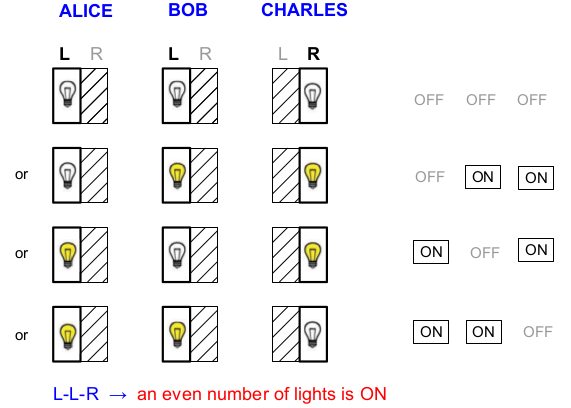
\includegraphics[scale=0.5]{ch2/image5.png}
	\captionof{figure}{Protons et antiprotons incidents sur une cible de silicium : le pouvoir 
	d'arrêt est plus important pour les protons que pour des antiprotons.}
\end{center}
\item[$\bullet$] \textit{Correction de Bloch}\ \\
Il s'agit du terme $z^2L_2(\beta)$, une correction pas très importante que l'on évalue généralement
avec l'évaluation de \textsc{Bichsel}
\begin{equation}
z^2L_2(y) = -y^2[1.202-y^2(1.042-0.855y^2+0.343y^4)]
\end{equation}
où $y=z\alpha/\beta$ avec $\alpha = 1/137$ le constante de structure fine.
\end{itemize}

\newpage
	\begin{wrapfigure}[11]{r}{9cm}
%	\vspace{-5mm}
	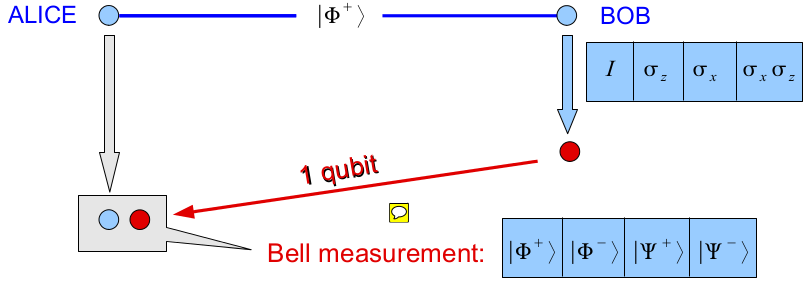
\includegraphics[scale=0.4]{ch2/image6.png}
	\captionof{figure}{ }
	\end{wrapfigure}
Évaluons maintenant les effets des différentes corrections. Le graphique ci-contre (à gauche) 
concerne des protons incidents sur une cible d'aluminium. On peut y voir que la correction de
\textsc{Bloch} (en bas à gauche) est vraiment très faible. A droite est représenté la correction
relative pour des protons incidents sur une cible d'or ($L_1$ concerne \textsc{Barkas} et $L_2$
\textsc{Bloch}).


\subsection{Petites vitesses}
Lorsque $v \lesssim v_0$, on ne peut plus appliquer la méthode des perturbations et il faut 
commencer à prendre en compte les captures électroniques par l'ion indicent (l'ion va si
lentement qu'il peut capturer un (ou plusieurs) électron) modifiant la charge $z^*$ de 
celui-ci. Par la théorie de \textsc{Thomas-Fermi}
\begin{equation}
z^*=z\left(1-e^{-v/(z^{2/3}v_0)}\right)
\end{equation}
Une technique consiste à considérer un état de charge moyen même si ce n'est pas vrai en tout 
point.


\section{Pouvoir d'arrêt nucléaire (faibles vitesses)}
Les effets étant tellement négligeable que nous ne rentrerons pas dans les détails ici. Comme
vu au premier chapitre, les collisions nucléaire pour des ions incidents sont rares et contribuent
peu au pouvoir d'arrêt total. Elle se produise presque exclusivement pour des ions incidents de 
faible vitesse et même alors leur contribution est faible. Cependant, elle peuvent avoir des effets
à postériori et causer des dégâts radiatifs.\\

	\begin{wrapfigure}[12]{r}{5.6cm}
	\vspace{-11mm}
	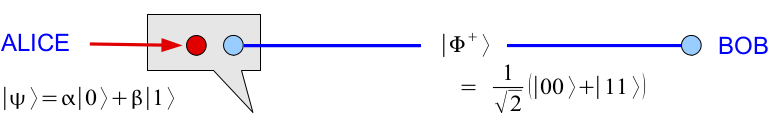
\includegraphics[scale=0.34]{ch2/image7.png}
	\captionof{figure}{ }
	\end{wrapfigure}
Plaçons-nous dans le système du centre de masses pour observer la diffusion par un angle 
$\theta$ due à un potentiel central $V(r)$. Reprenons la formule générale pour la section efficace
d'arrêt 
\begin{equation}
S_n = \int Td\sigma = \int T 2\pi p dp = 2\pi\gamma E\int \sin^2(\theta/2)pdp
\end{equation}
où $\gamma = \frac{4m_1m_2}{(m_1+m_2)^2}$. Pour le calculer, il est nécessaire de connaître $\theta$
ce qui peut se faire avec le schéma avec une particule incidente et cible représenté ci-contre.\\

Pour évaluer $\theta$, on utilise l'équation de la variation angulaire en coordonnée sphérique tout
en introduisant le potentiel. 

\begin{eqnarray*}
\frac{m_0}{2}\left[ \left( \frac{dr}{dt}\right)^2+r^2\left( \frac{d\varphi}{dt}\right)^{2}\right]+V(r)=\frac{m_0}{2}v^2\equiv E_r\\
m_0r^2\frac{d\varphi}{dt}=-m_0pv
\end{eqnarray*}
On en tire
\begin{equation}
\theta=\pi-2\int_{r_{m}}^\infty dr \frac{p}{r^2}\left( 1-\frac{V(r)}{E_r}-\frac{p^2}{r^2}\right)^{-1/2}
\end{equation}


Il faut maintenant spécifier le potentiel. Le plus logique serait d'utiliser celui de \textsc{Coulomb}
mais sa variation en $1/r$ cause une divergence du paramètre d'impact à cause de la portée infinie. 
Comme il y a toujours interaction, on va préférer considérer un effet d'écrantage par les électrons
atomiques qui diminue la portée du potentiel. Pour se faire, on va simplement introduire une 
exponentielle décroissante $\exp(-r/r_s)$.\\

Pour un modèle plus précis, on peut insérer une fonction $F_s(r/r_s)$. Le potentiel d'interaction 
devient alors
\begin{equation}
V(r)=\frac{z_1Z_2e^2}{r}F_s(\frac{r}{r_s})
\end{equation}
Il s'agit de la \textit{fonction d'écrantage universelle}, obtenue par ajustement aux résultats 
expérimentaux.\\

	\begin{wrapfigure}[12]{r}{5.6cm}
	\vspace{-11mm}
	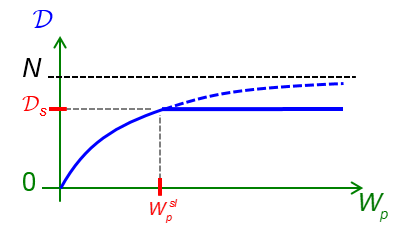
\includegraphics[scale=0.34]{ch2/image8.png}
	\captionof{figure}{ }
	\end{wrapfigure}
Mettons maintenant ces effets ensemble en considérant des protons incidents sur une cible 
d'aluminium comme représenté ci-contre. Nous avons $S = S_{elec} + S_{nucl} \approx S_{elec} 
= S_{coll}$. On voit que l'effet du pouvoir d'arrêt nucléaire est très faible, on retrouve
le plateau de Fermi à grande vitesse et une pente ou la formule de \textsc{Bohr} est valable.


\section{Pouvoir d'arrêt massique électronique et influence de la phase}
Par définition, le pouvoir d'arrêt massique d'un matériau est le rapport du pouvoir d'arrêt 
linéique et de lamasse volumique $\rho$ de ce matériau (unités usuelle : MeV.cm$^2$.g$^{-1}$. 
\begin{equation}
\frac{NS(E)}{\rho}=-\frac{1}{\rho}\frac{dE}{dx}
\end{equation}
Comme $\rho = M_AN/N_A$ où $M_A=AM_u$, en divisant des deux côtés par cette même quantité on 
trouve\\

\cadre{\begin{equation}
-\dfrac{1}{\rho}\dfrac{dE_{elec}}{dx} = 4\pi r_e^2mc^2\frac{N_A}{M_u}\dfrac{Z}{A}\dfrac{z^2}{\beta^2}
L(\beta)
\end{equation}}\ \\

Passons en revue les quatre facteurs du pouvoir d'arrêt massique électronique
\begin{enumerate}
\item Le facteur constant $4\pi r_e^2mc^2N_A/M_u = 0.307$ MeV.cm$^2$.g$^{-1}$ qui donne l'ordre
de grandeur de ce pouvoir
\item Le facteur $Z/A$ compris entre 0.4 et 0.5 pour tout les isotopes stable (sauf $H$). Comme
c'est le terme principal de dépendance du matériau et que celui-ci est $\pm$ constant la dépendance
du matériau est faible : c'est l'intérêt de cette formule
\item Le facteur $\beta^{-2}$ est une fonction monotone décroissante de la vitesse de l'ion qui
tend vers 1 pour les grandes énergies. Ce-dernier explique la diminution du pouvoir d'arrêt 
avec l'énergie. 
\item Le nombre d'arrêt $L(\beta)$ est une fonction monotone croissante (lente) de la vitesse 
et de $Z$.
\end{enumerate}

\subsection*{Influence de la phase}
Aux grandes énergies, la correction de densité influe impliquant une grande correction de phase 
dans les solides et faible dans les gaz. Aux faibles énergies il faut tenir compte de l'influence
des liaisons chimiques et intermoléculaires ce qui se traduit par une modification de la
valeur de $I$.

\section{Parcours et courbe de Bragg} 
\subsection{Parcours}
Lorsque les particules \textbf{chargées} perdent leur énergie dans la matière, elles parcourent une
certaine distance dans la matière mais celle-ci peut être variable a cause des pertes d'énergies 
et des déviations aléatoires (\textit{starggling}). Il faut alors définir plusieurs parcours
\begin{itemize}
\item[$\bullet$] Le parcours $R$ d'une particule chargée d'énergie $E$ dans un milieu et 
la valeur moyenne $\langle l \rangle$ de la longueur $m$ de sa trajectoire suivie jusqu'à son 
arrêt (en négligeant le mouvement thermique)
\item[$\bullet$] Le parcours projeté $R_p$ d'une particule chargée d'énergie $E$ dans un milieu. 
Celui-ci correspond à la valeur moyenne de sa profondeur de pénétration $\langle d \rangle$ dans la
direction initiale de la particule.
\end{itemize}
A cause du caractère sinueux des trajectoires, $R_r<R$. On défini alors le \textbf{facteur de détour}
$R_p/R_{CSDA} < 1$.\\

Dans l'approximation $CSDA$
\begin{equation}
R_{CSDA}=\int^{E}_{0}\frac{dE'}{NS(E')}
\end{equation}
En remplaçant $S$ par l'expression de \textsc{Bethe} (non-relativiste, avec $dE=Mv$d$v$)
\begin{equation}
R_{CSDA}\propto \int^{v}_{0}\frac{v^3dv}{L(v)}
\end{equation}
En négligeant la dépendance en la vitesse du nombre d'arrêt 
\begin{equation}
R_{CSDA}\propto v^4\propto E^2
\end{equation}
En réalité, l'équation de \textsc{Bethe} (ou \textsc{Bethe-Bloch}) n'est pas valable à faibles
vitesses et il faut nécessairement passer par de faibles vitesses pour s'arrêter. On utilisera 
alors la formule empirique suivante
\begin{equation}
\rho R_{CSDA}=\frac{E^{1.77}}{415}+\frac{1}{670}
\end{equation}

\subsubsection{Considérations sur le parcours}
Reprenons l'approximation $NS(E)\propto 1/E$. Soit une particule incidente de masse $M_i$ et de
charge $z_i$
\begin{equation}
NS(E)=-\frac{dE}{dx} \Rightarrow -\frac{M_i}{z_i^2}\frac{dv^2}{dx}\propto \frac{1}{v^2}
\end{equation}
Pour deux particules incidentes $(M_1,z_1)$ et $(M_2, z_2)$ de même vitesse initiale
\begin{equation}
\frac{R_{CSDA}^1}{R_{CSDA}^2}=\frac{M_1z_2^2}{M_2z_1^2}
\end{equation}
Il s'agit d'une petite formule utile pour estimer l'ordre de grandeur qui nous informe que le range
pour des protons et des $\alpha$ de même vitesse est similaire.


\subsection{Courbes de Bragg}
Soit un milieu semi-infini et un faisceau parallèles de particules chargées identiques et de même
énergie : toutes les particules vont forcément s'arrêter, après une distance $R_{CSDA}$. La 
courbe de \textsc{Bragg} donne la \textbf{dose} (énergie moyenne déposée par unité de masse de la
cible) déposée par la particule chargée en fonction de la profondeur. \\

A une profondeur $x$, la particule doit encore parcourir $d=R_{CSDA}-x$. Comme l'énergie déposée
$D \propto S \propto 1/v^2$, cela implique que $R_{CSDA}\propto v^4$. Dès lors
\begin{equation}
D\propto \frac{1}{\sqrt d}=\frac{1}{\sqrt{R_{CSDA}-x}}
\end{equation}

	\begin{wrapfigure}[12]{r}{8.5cm}
	\vspace{-7mm}
	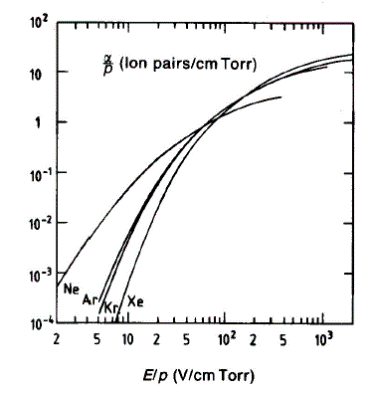
\includegraphics[scale=0.5]{ch2/image9.png}
	\captionof{figure}{Protons de 700 MeV dans de l'eau}
	\end{wrapfigure}
Ceci a des applications en protonthérapie (ou hadronthérapie). Lorsque l'on a une tumeur, il faut
la soumettre à un rayonnement pour l'éliminer. On pourrait envoyer des électrons, mais entre la 
tumeur et la peau il y a pas mal de choses qu'il ne vaut mieux pas endommager et le problème est que 
les électrons vont déposer pas mal d'énergie entre les deux. Avec la protonthérapie, la zone dans 
laquelle il ne faut pas déposer l'énergie sera faible et le maximum d'énergie sera déposé la ou 
la tumeur se situe.\\

\subsection*{Interactions nucléaires fortes}
	\begin{wrapfigure}[5]{l}{3cm}
	\vspace{-7mm}
	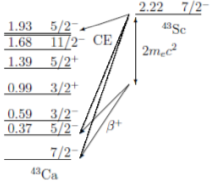
\includegraphics[scale=1.5]{ch2/image10.png}
%M	\captionof{figure}{ }
	\end{wrapfigure}
Lorsqu'un ion s'approche très près d'un noyau, une interaction nucléaire forte est possible et le
noyau peut être brisé. Par exemple, en fragmentant le plomb on aura un excès de neutron. Ce 
processus de production de neutrons est nomme \textit{spallation}. Le projet \textit{Myrrha} se
base la dessus. L'idée est de faire un réacteur avec un accélérateur en envoyant des protons sur
du Pb pour produire des neutrons et après se trouve un réacteur classique : pour l'arrêter, il suffit
de couper l'accélérateur.
\chapter{Bruits et parasites}
Introduisons la notion de  bruit et parasite:
\begin{description}
	\item[Bruit] au sens strict (encore appelé "bruit de fond") est un signal à variation aléatoire d'origine \emph{interne} au dispositif étudié. Il est possible de le définir, de prévoir son niveau plancher à l'aide du dimensionnement
	\item[Parasites] signaux perturbateurs d'origine \emph{externe} au dispositif
\end{description}
Ces 2 phénomènes se présentent sous forme de signal analogique venant s'additionner au signal utile, entraînant ainsi sa dégradation. Une fois le signal utile perturbé, pas de marche arrière, d'où l'importance des ces concepts lors du dimensionnement.
\begin{table}[H]
	\centering
	\begin{tabular}{lcr}
		& \textbf{bruit} & \textbf{parasite} \\ \hline
		origine & interne & externe \\
		distribution & aléatoire & variable \\
		bande passante & "\(\infty\)" & limitée \\
		amplitude & faible & variable \\
		& "plancher" & arbitrairement bas \\
		modélisation & "facile" & difficile \\
		contre-mesures & conception & conception/remédiation \\ \hline
 	\end{tabular}
	\caption{Critères de distinction}
\end{table}
On remarque que:
\begin{itemize}
	\item contrairement au bruit qui possède généralement une amplitude plancher, calculable théoriquement, il est théoriquement impossible de réduire les parasites à un niveau arbitrairement bas.
	\item La modélisation des effets du bruit dans un système est, dans le principe, simple. Au contraire, la modélisation des parasites est nettement plus difficile car ceux-ci sont constitués de plusieurs signaux plus déterministes dont il faut connaître les couplages avec le système étudié.
\end{itemize}
L'introduction des ces phénomènes relève tout l'intérêt des signaux numérique (au lieu d'analogique). En effet, alors qu'un signal analogique dégradé ne peut être restauré, il est possible généralement de restaurer un signal numérique dégradé.\\
Un signal numérique n'est rien d'autre qu'un signal analogique dont certains niveaux représentent des valeurs discrètes portant une information (paliers, ex. 0=vrai, 1=faux) et dont chaque niveau peut varier dans certaines limite \(\rightarrow\) marges de bruit.\\

Ainsi, si l'impact des bruits et parasites est inférieur à cette marge de bruit définie par la conception, il est possible de restaurer le signal numérique utile. Les signaux numériques présentent donc une meilleure robustesse face aux perturbations. Il sera néanmoins toujours nécessaire de limiter les perturbations (car marges de bruit limitées).
\section{Le bruit de fond}
\subsection{Introduction}
Le bruit de fond possède plusieurs caractéristiques:
\begin{itemize}
	\item fluctuation aléatoire fondamentale due à la nature elle-même du dispositif
	\item limite ultime de la résolution du dispositif (contrairement aux parasites)
	\item fondamentalement inévitable (jamais nul) mais son influence sur la chaîne peut être minimisée
	\item origine générale en électronique: fluctuations de la densité des porteurs de charges (porteurs de charges = \(e^-\) et trous, fonction de la température)
	\item observable sur une tension et/ou un courant
\end{itemize}
Il existe plusieurs type de bruit, comme le bruit de type gaussien (c-à-d qui suit une loi normale de moyenne et variance données \(N(\mu,\sigma)\), \autoref{fig:densiteprobagauss})

\begin{figure}[H] 
	\centering 
\pgfmathdeclarefunction{gauss}{2}{%
	\pgfmathparse{1/(#2*sqrt(2*pi))*exp(-((x-#1)^2)/(2*#2^2))}%
}
	\begin{tikzpicture}[
	scale=0.6,
	every pin edge/.style={<-},
	every pin/.style={fill=yellow!50,rectangle,rounded corners=3pt,font=\small}]
	\begin{axis}[every axis plot post/.append style={
		mark=none,domain=-3:3,samples=30,smooth},
	clip=false,
	axis y line=none,
	axis x line*=bottom,
	ymin=0,
	xtick=\empty,
	]
	\addplot {gauss(0,0.5)};
	\addplot {gauss(0,1)};
	\draw[dashed]  (axis description cs:0.5,0) node[below] {\(\mu\)} -- (axis description cs:0.5,0.92) ;
	\end{axis}
	\end{tikzpicture}
\caption{Bruit de type gaussien: densité de probabilité}
\label{fig:densiteprobagauss}
\end{figure}
Valeur maximale du bruit ? Prenons un bruit de valeur efficace \(\SI{1}{\volt}\) (\autoref{fig:tensionbruitmax}). Il est tout à fait possible qu'au bout de \(\SI{100}{\second}\) on ait un bruit 10 fois plus grand. C'est aléatoire, mais sa puissance rms est constante.
\begin{figure}[H] 
	\centering 
	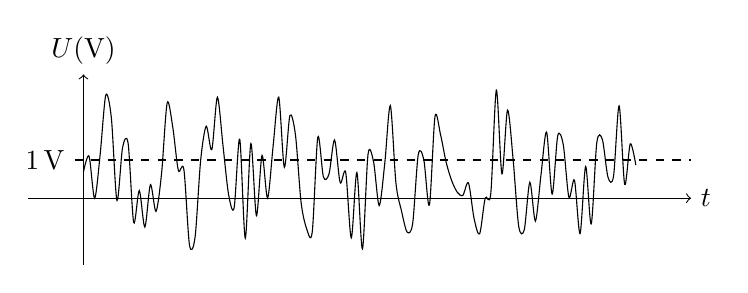
\begin{tikzpicture}[samples=100, domain=0:5*360]
	\begin{axis}[
	width=10cm, height=4cm,
	enlarge x limits=true,
	xtick=\empty,
	ytick=\empty,
	axis line style={->},
	axis lines*=middle,
	xlabel=\(t\),
	ylabel=\(U(\si{\volt})\),
	every axis x label/.style={
		at={(ticklabel* cs:1)},
		anchor=west,
	},
	every axis y label/.style={
		at={(ticklabel* cs:1)},
		anchor=south,
	},]
	\addplot [no markers, smooth] {sin(x)*sin(x)+rand};
	\draw[dashed] (axis description cs:0.07,0.55) node[left] {\SI{1}{\volt}} -- (axis description cs:1,0.55) ;
		\end{axis}
	\end{tikzpicture}
	\caption{Bruit de type gaussien: tension} 
	\label{fig:tensionbruitmax}
\end{figure}

\paragraph{Remarque:} la "valeur efficace" est une puissance mesurée, ce n'est pas le max
\subsection{Caractérisation mathématique}
\subsubsection{Définition de base}
Mathématiquement, le bruit est caractérisé par un \emph{signal temporel} (f.e.m) \(E_b(t)\) avec les propriétés suivantes:
\begin{itemize}
	\item {\makebox[8cm]{fluctuation aléatoire \(\Rightarrow\) moyenne nulle\hfill} \(\overline{E_b(t)}=0\)}
	\item {\makebox[8cm]{valeur quadratique moyenne non nulle\hfill} \(\overline{E_b^2(t)} \neq 0\)}
	\item {\makebox[8cm]{valeur efficace ("rms" = root mean square)\hfill} \(E_b=\sqrt{\overline{E_b^2(t)}}\)}
	\item {\makebox[8cm]{rapport signal/bruit SNR [dB]\hfill} \(SNR=10\log\left(\overline{E^2_s(t)}/\overline{E_b^2(t)}\right)\)}
\end{itemize}
\subsubsection{Variation en fréquence}
À ces propriétés s'ajoutent:\begin{itemize}
	\item La valeur efficace dépend de la fréquence \(\Rightarrow\) \emph{densité spectrale} de bruit \[e_b(f)=\sqrt{\left.\frac{d\overline{E_b^2}}{df}\right|_f}\quad [\si[per-mode=symbol]{\volt\per\sqrt{\hertz}}]\]
	\item La couleur du bruit:
	\begin{itemize}
		\item bruit blanc: densité spectrale constante en fréquence (uniformément réparti en fréquence, \autoref{fig:bruitblanc})
		\item bruit rose: densité spectrale plus forte pour les basses fréquences (descente linéaire, \autoref{fig:bruitrose})
	\end{itemize}
\end{itemize}
\begin{figure}[H]
	\centering
	\subfigure[Bruit blanc]{\label{fig:bruitblanc}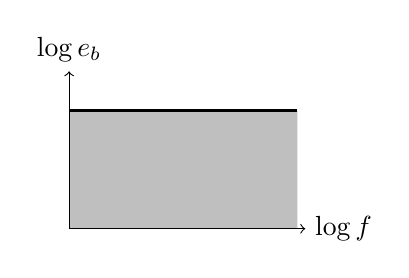
\begin{tikzpicture}
		\fill [gray!50, domain=0:2.9, variable=\x]
		(0, 0)
		-- plot ({\x}, {1.5})
		-- (2.9, 0)
		-- cycle;
		\draw[->] (0,0) -- (0,2) node[above]{\(\log e_b\)};
		\draw[->] (0,0) -- (3,0) node[right]{\(\log f\)};
		\draw[very thick] (0,1.5) -- (2.9,1.5);
		\end{tikzpicture}}
	\subfigure[Bruit rose]{\label{fig:bruitrose}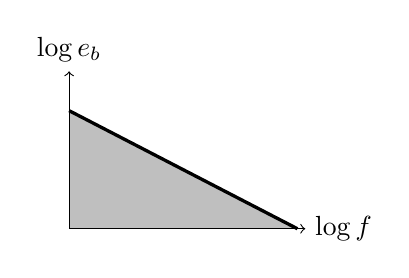
\begin{tikzpicture}
		\fill [gray!50, domain=0:2.9, variable=\x]
		(0, 0)
		-- plot ({\x}, {1.5-\x*0.51})
		-- (2.9, 0)
		-- cycle;
		\draw[->] (0,0) -- (0,2) node[above]{\(\log e_b\)};
		\draw[->] (0,0) -- (3,0) node[right]{\(\log f\)};
		\draw[very thick] (0,1.5) -- (2.9,0);
		\end{tikzpicture}}
	\caption{Répartition en fréquence de la densité spectrale de bruit}
\end{figure}
\subsubsection{Sommation de bruits divers}
Dans l'hypothèse où il n'y a pas corrélation entre:
\begin{itemize}
	\item les sources de bruits d'origine différente
	\item la même source à différentes fréquences
\end{itemize}
\centerline{\(\Rightarrow\) Puissance totale de bruit = \(\sum\) des puissance de bruit individuelles.}
Or la puissance de bruit \(\propto\) valeur quadratique moyenne de la tension ou du courant de bruit \(\rightarrow P_b=R \overline{I^2_b} = \frac{\overline{V_b^2}}{R}\). Il faut donc sommer \emph{quadratiquement} tensions et courants de bruit 
\[
V_b^2 = V_{b_1}^2 + V_{b_2}^2 + \dots + V_{b_n}^2 \qquad I_b^2 = I_{b_1}^2 + I_{b_2}^2 + \dots + I_{b_n}^2
\]
De même pour les densités spectrales:
\[
v_b^2(f) = v_{b_1}^2(f) + v_{b_2}^2(f) + \dots + v_{b_n}^2(f)
\]
\subsection{Types de bruit}
\subsubsection{Bruit thermique ou de Johnson}
Le bruit thermique est un bruit dû à l'agitation thermique des porteurs de charges (\(e^-\) dans conducteur, \(e^-+\) trous dans semi-conducteur). À \(T>\SI{0}{\kelvin}\), il y a collision des porteurs de charges entre eux \(\rightarrow\) répartition non uniforme des charges électriques \(\rightarrow\) champ électrique variable aléatoirement.\bigbreak

Ses propriétés sont les suivantes:
\begin{itemize}
	\item {\makebox[6cm]{valeur moyenne nulle\hfill} \(\overline{E_{bR}(t)}=0\)} 
	\item {\makebox[6cm]{valeur quadratique moyenne\hfill} \(\overline{E^2_{bR}(t)}=4kRT\Delta f\)} avec \(\left\{\substack{k\text{ : cst de Boltzmann }=\SI[per-mode=symbol]{1.374e-23}{\joule\per\kelvin}\\
	R \text{ : résistance en }\si{\ohm}\hfill \\
	T\text{ : température absolue en }\si{\kelvin}\hfill\\
	\Delta f\text{ : bande de fréquence observée}\hfill}\right.\)
	\item bruit blanc
	\item existe dans toute résistance vraie
	\item mesurable malgré son faible ordre de grandeur\footnote{Potentiel du cerveau \(\approx \SI{1}{\micro\volt}\)}
\end{itemize}
\subsubsection{Bruits en 1/f}
Les bruits en 1/f sont plus fort à basses qu'à hautes fréquences (bruit rose), il en existe 2 types:
\begin{itemize}
	\item Bruit de scintillation:
	\begin{itemize}
		\item présent dans les semi-conducteurs
		\item d'origine incertaine, recombinaisons dans les défauts de surface du semi-conducteur (\(e^-\) et trous)
	\end{itemize}
	\item Bruit en excès (ou bruit de constitution, "contact noise", "excess noise"):
	\begin{itemize}
		\item analogue au bruit de scintillation
		\item présent dans certaines résistances (ex. résistance à couche de carbones)
		\item engendré par l'évolution erratique (:= aléatoire) des lignes de courant (continu) dans un matériau non homogène
	\end{itemize}
\end{itemize}
\subsubsection{Autres types de bruit}
Le reste:
\begin{itemize}
	\item Bruit de grenaille (ou de Schottky):
	\begin{itemize}
		\item présent dans les semi-conducteurs
		\item dû à la nature quantifié du courant électrique, provoqué par passage des porteurs de charge au travers d'une barrière de potentiel
	\end{itemize}
	\item Bruit quantique:
	\begin{itemize}
		\item dû à la nature quantifiée de l'énergie rayonnée (photons)
	\end{itemize}
	\item Bruit de diffusion:
	\begin{itemize}
		\item présent dans les semi-conducteurs
		\item dû aux collisions des porteurs de charges avec le réseau cristallin
	\end{itemize}
	\item Bruit de génération/recombinaison:
	\begin{itemize}
		\item présent dans les semi-conducteurs
		\item  dû à la fluctuation aléatoire des taux de génération, des recombinaisons et des piégeages des porteurs
	\end{itemize}
	\item Bruit d'avalanche:
	\begin{itemize}
		\item présent dans les diodes Zener à tension d'avalanche élevée
		\item  dû au délogement de certains \(e^-\) à cause d'\(e^-\) accélérés par le champ électrique, venant créer des porteurs de charge supplémentaires (bruit important au voisinage de l'effet d'avalanche)
	\end{itemize}
	\item Bruit d'éclatement (ou bruit impulsif, "burst noise", "popcorn noise"):
	\begin{itemize}
		\item présent dans certains dispositifs électronique particulier (ex. diode tunnel)
		\item d'origine incertaine, lié aux défauts de fabrication
		\item Bruit non gaussien
	\end{itemize}
\end{itemize}
\subsection{Modélisation de bruit}
\paragraph{Dans un résistance:} la \autoref{fig:bruitresist} représente l'équivalent de Thévenin et de Norton pour le bruit thermique.
\begin{figure}[H] 
	\centering 
	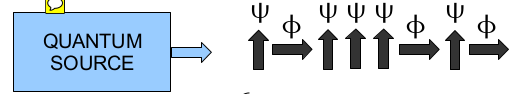
\includegraphics[width=0.8\textwidth,height=10\baselineskip,keepaspectratio]{ch3/image1} 
	\caption{Bruit thermique dans une résistance}
	\label{fig:bruitresist}
\end{figure}
\paragraph{Dans un transistor:} rappelons qu'un amplificateur différentiel est constitué de transistors. Les sources de bruits sont:
\begin{itemize}
	\item bruit thermique des résistances vraies (\(R_{BB}'\))
	\item bruit de grenaille des courants (base et collecteur)
	\item bruit en 1/f du transistor
\end{itemize}
La modélisation du bruit est présenté à la \autoref{fig:bruittrans}.
\begin{figure}[H] 
	\centering 
	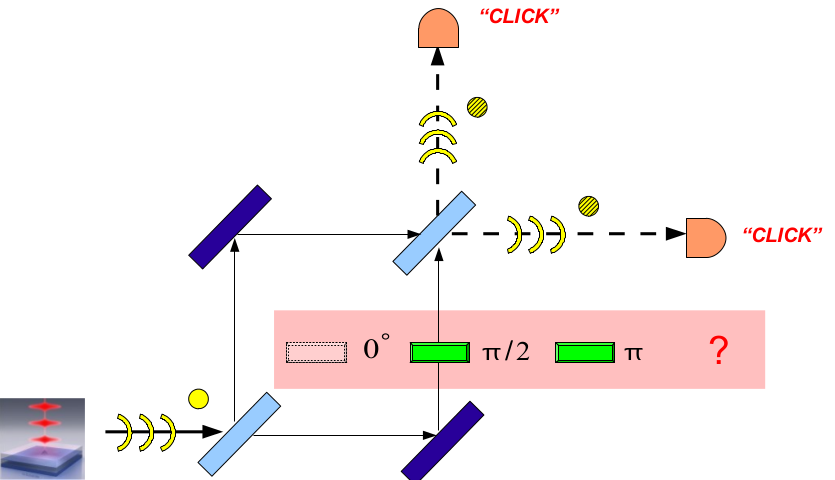
\includegraphics[width=0.4\textwidth,height=10\baselineskip,keepaspectratio]{ch3/image2} 
	\caption{Bruit dans un transistor}
	\label{fig:bruittrans}
\end{figure}
\paragraph{Dans un AOP:} rappelons qu'on AOP est constitué de résistances et de transistors. Le bruit est modélisé par la \autoref{fig:bruitaop}.
\begin{figure}[H] 
	\centering 
	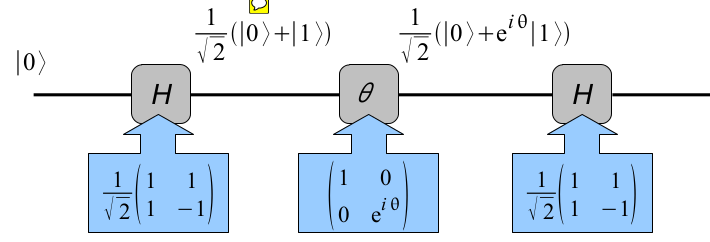
\includegraphics[width=0.8\textwidth,height=10\baselineskip,keepaspectratio]{ch3/image3} 
	\caption{Bruit dans un amplificateur opérationnel} 
	\label{fig:bruitaop}
\end{figure}
\paragraph{Remarques:} Les courants \(i_{b^\pm} \neq\) courant de bias (= courant constant de polarisation). \(i_{b^\pm}\) sont des courants à moyenne nulle, allant vers le circuit et dont l'impact dépend de l'impédance (+ l'impédance est grande, + le bruit est grand).
\subsection{Limitation de bruit}
\subsubsection{Introduction et principales techniques}
Le but de cette sous-section est de développer des méthodes afin de rendre l'amplitude du bruit négligeable face à celle du signal, c-à-d \(\nearrow\) SNR. Pour ce faire, il est possible d'agir sur 2 choses:
\begin{enumerate}
	\item Augmenter le signal, c-à-d amplifier dès que possible et autant que possible le signal \(\Rightarrow\) pré-ampli à grand gain et faible bruit.
	\item Réduire le bruit de tous les composants.
\end{enumerate}
Afin de parvenir à un résultat, il est important de suivre ces quelques règles de base:
\begin{enumerate}
	\item Cibler le type de bruit (afin de choisir des contre-mesures efficaces).
	\item S'attaquer au bruit prépondérant (on va peut-être s'occuper du gros d'abord, non ?).
	\item S'attaquer au bruit dès que possible (chaque module apportant son propre bruit (irréversible), il devient impossible de séparer les bruits entre eux au fur et à mesure que l'on avance sur la chaîne)
\end{enumerate}
Nous pouvons agir:
\begin{description}
\item \emph{Au niveau des composants:}
\begin{itemize}
	\item Choisir des composants à faible bruit.
	\item Jouer sur les paramètres influençant directement le bruit (ex. réduire la température pour un bruit thermique).
\end{itemize}
\item \emph{Au niveau du système:}
\begin{itemize}
	\item \hyperref[subsubsec:entreenobruit]{Pré-ampli à faible bruit} (parfois étage à transistor discrets afin de minimiser le bruit de l'aop, lui-même constitué d'un nombre conséquent de transistors discrets).
	\item \nameref{subsubsec:bandepass} (réduire le bruit dans un bande passante plus restreinte).
	\item \nameref{subsubsec:résistsource}.
	\item \nameref{subsubsec:detectsync} pour le bruit rose.
\end{itemize}
\end{description}
\subsubsection{Réduire la bande passante} \label{subsubsec:bandepass}
Le bruit à virtuellement une bande passante infinie alors que celle du dispositif de mesure est limitée \(\Rightarrow\) bruit perçu limité à la bande passante du dispositif.\bigbreak

Pour un bruit blanc de densité \(e_{bb}\) perçu au travers d'une bande passante \(B=f_{\text{max}}-f_{\text{min}}\):
\begin{equation}
E_b^2 = \int_{f_{\text{min}}}^{f_{\text{max}}} dE_b^2 = \int_{f_{\text{min}}}^{f_{\text{max}}} e_{bb}^2\,df = e_{bb}^2(f_{\text{max}}-f_{\text{min}}) 
\end{equation}
Ainsi, la valeur efficace du bruit dans une bande de fréquence, permettant d'avoir une idée sur l'amplitude du bruit, est:
\begin{equation}\label{eq:valeffbruitDB}
E_b = e_{bb}\sqrt{B}
\end{equation}
On déduit de \eqref{eq:valeffbruitDB} que plus la bande passante du dispositif de mesure \(\nearrow\), plus le bruit présent à la sortie de la chaîne de mesure \(\nearrow\) et donc plus le signal est perturbé. \(\Rightarrow\) Il faut \textbf{limiter la bande passante} (filtrage).\bigbreak

Dans un dispositif réel, le bruit est un "bruit composite" (rose (aux basses fréquences) + blanc (aux hautes fréquences)). Le point où les 2 densités spectrales sont égales (rose \(\cup\) blanc) est appelé la \emph{fréquence coin}.
\begin{figure}[H]
	\centering
	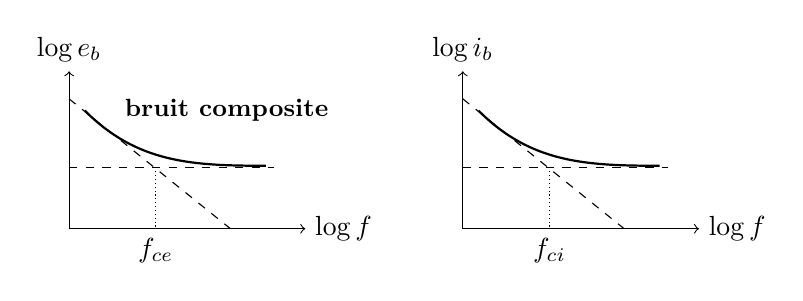
\begin{tikzpicture}
		\draw[dashed] (0,1.65) -- (2.05,0);
		\draw[dashed] (0,0.78) -- (2.6,0.78);
		\draw[densely dotted] (1.1,0.78) -- (1.1,0) node[below]{\(f_{ce}\)};
		\draw[thick] (0.2,1.5) to[out=-45, in=180] (2.5,0.8);
		\draw[->] (0,0) -- (0,2) node[above]{\(\log e_b\)};
		\draw[->] (0,0) -- (3,0) node[right]{\(\log f\)};
		\draw (2,1.5) node{\textbf{\small bruit composite}};
		\draw[dashed] (5,1.65) -- (7.05,0);
		\draw[dashed] (5,0.78) -- (7.6,0.78);
		\draw[densely dotted] (6.1,0.78) -- (6.1,0) node[below]{\(f_{ci}\)};
		\draw[thick] (5.2,1.5) to[out=-45, in=180] (7.5,0.8);
		\draw[->] (5,0) -- (5,2) node[above]{\(\log i_b\)};
		\draw[->] (5,0) -- (8,0) node[right]{\(\log f\)};
		\end{tikzpicture}
\end{figure}
La valeur efficace de bruit composite dans la bande passante est :
\begin{equation}
E_b^2 = e_{bb}^2\left[(f_{\text{max}}-f_{\text{min}})+f_{ce}\ln\left(\frac{f_{\text{max}}}{f_{\text{min}}}\right)\right]
\end{equation}
Ainsi, pour réduire le bruit il faut:
\begin{itemize}
	\item limiter la bande passante (\(f_{\text{max}}-f_{\text{min}}\))
	\item choisir des composants pour minimiser:
	\begin{itemize}
		\item la densité spectrale de bruit blanc \(e_{bb}\text{ (et }i_{bb}\))
		\item la fréquence de coupure \(f_{ce}\text{ (et }f_{ci}\))
	\end{itemize}
\end{itemize}
\subsubsection{Résistance de source} \label{subsubsec:résistsource}
\begin{description}
	\item[\(R_s\)] résistance de sortie du capteur (ou de l'étage précédent)
\end{description}
Un AOP comprend des sources de tension de bruit et de courant de bruit, il faut donc choisir un ampli à:
\begin{itemize}
	\item faible tension de bruit lorsque \(R_s\) est faible
	\item faible courant de bruit lorsque \(R_s\) est élevée
\end{itemize}
\subsubsection{Étage d'entrée à faible bruit} \label{subsubsec:entreenobruit}
Comparons 2 cas possible d'étage d'entrée de gain total \(G\):\bigbreak
\underline{Amplificateur unique:}  soit sa densité spectrale de bruit ramené à l'entrée \(v_b^{in}\), le bruit total à la sortie vaut
\begin{equation}\label{eq:etasortieunique}
v_b^{out}=G . v_b^{in}
\end{equation}
\underline{Ajout d'un étage d'entrée à faible bruit:} soit un 1\up{er} étage d'entrée de gain \(G_1\) et de densité spectrale de bruit (entrée) \(v_{b_1}^{in}\) et un 2\up{ème} étage de gain \(G_2\) et de densité spectrale de bruit (entrée) \(v_{b_2}^{in}\) tel que \(G_1 . G_2 = G\). Nous aurons donc à la sortie du premier étage:
\begin{itemize}
	\item le bruit dû au 1\up{er} étage: \(v_{b_1}^{out}=G_1 . v_{b_1}^{in}\)
	\item le bruit dû au 2\up{ème} étage: \(v_{b_2}^{in}\)
\end{itemize}
Et donc, le bruit total à la sortie vaut:
\begin{equation}\label{eq:etasortie}
v_b^{out} = G_2\sqrt{\left(v_{b_1}^{out}\right)^2 + \left(v_{b_2}^{in}\right)^2} = G\sqrt{\left(v_{b_1}^{in}\right)^2 + \left(v_{b_2}^{in}/G_1\right)^2}
\end{equation}
On remarque que le bruit total de \eqref{eq:etasortie} sera plus faible que celui de \eqref{eq:etasortieunique} si \(G_1\gg 1\text{ et } v_{b_1}^{in}<v_b^{in}\)
\begin{center}
	\textbf{le bruit d'un ampli est minimisé en plaçant en tête un préamplificateur à faible bruit et de gain suffisant}
\end{center}
\subsubsection{Détection synchrone} \label{subsubsec:detectsync}
Si le signal utile se situe à basse fréquence, le bruit en 1/f (rose) domine \(\Rightarrow\) transposer momentanément le signal utile à une fréquence plus élevée, à l'aide d'une modulation d'amplitude (signal sera au alentour de la fréquence porteuse), afin de réaliser la transmission ou l'amplification en dehors de la bande bruitée. 
\begin{figure}[H] 
	\centering 
	\begin{tikzpicture}
	 	\draw plot[domain=0:3*pi] (\x,{0.6*sin(\x r)}) node[right]{signal};
	 	\draw plot[samples=300,domain=0:3*pi] (\x,{0.6*sin(20*\x r)*(1+0.6*sin(\x r)) -2}) node[right]{AM};
	 	\node[draw,ellipse] (C) at (-0.5,-4){capteur};
	 	\node[draw] (M) at (2.5,-4){modulation};
	 	\node[draw] (A) at (5,-4){ampli};
	 	\node[draw] (D) at (7.5,-4){démodulation};
	 	\node[draw] (P) at (10.5,-4){Passe-bas};
	 	\draw[->, >=latex'] (C) -- (M);
	 	\draw[->, >=latex'] (M) -- (A);
	 	\draw[->, >=latex'] (A) -- (D);
	 	\draw[->, >=latex'] (D) -- (P);
	\end{tikzpicture} 
	\caption{Détection synchrone} 
\end{figure}
Pour résumer:
\begin{itemize}
		\item {\makebox[4cm]{signal utile:\hfill} \(s(t)\)}
		\item {\makebox[4cm]{signal modulation:\hfill} \(u_{mod}(t)=\cos(2\pi f_ut)\)}
		\item {\makebox[4cm]{signal démodulation:\hfill} \(u_{demod}(t) = \cos(2\pi f_ut+\varphi)\)}
\end{itemize}\ \\
Et donc, le signal modulé vaut:
\begin{equation}
s_{mod}(t) = s(t) . u_{mod}(t)
\end{equation}
qui est bien transposé autour de la fréquence \(f_u\) (\(f_u\gg f_{max}\)). Pour démoduler, nous utilisons une démodulation synchrone, c-à-d en multipliant par la même sinusoïde que lors de la modulation (+ déphasage inévitable \(\varphi\))
\begin{equation}
\begin{split}
s_{demod}(t) &= s_{mod}(t) . u_{demod}(t)\\
&= s(t)\cos(2\pi f_u t)\cos(2\pi f_u t+\varphi)\\
&= s(t)\frac{1}{2}\{\underbrace{\cos\varphi}_{\cst}+\cos(4\pi f_u t+\varphi)\}
\end{split}
\end{equation}
qui, après un filtre passe-bas (\(f_c \approx f_{max}\)) devient:
\begin{equation}
s_{demod}'(t) = s(t)\frac{\cos\varphi}{2}
\end{equation}
\section{Les parasites}
\subsection{Introduction}
Les parasites sont des tensions ou courants indésirables, d'origine extérieure à l'appareil perturbé, se superposant au signal utile. Ceux-ci apparaissent par suite du couplage d'un circuit source avec le circuit perturbé (victime).\bigbreak

L'origine physique le plus courant de ces parasites sont les parasites électromagnétiques (expliqués par les équations de Maxwell). Toutes charges et courants génèrent des champs (\(E\) et \(H\) variables, formant une onde électromagnétique) qui se transforment en f.e.m. (\(\int E\) ou \(H\) loi de Lenz). Il existe néanmoins d'autres phénomènes physiques comme la thermoélectricité, la piézoélectricité, etc.\bigbreak

À cela se rajoute le concept de champ proche et champ lointain ainsi que le type de couplages (C.f \autoref{fig:champproloin} et \autoref{fig:typcouplage})
\begin{figure}[H] 
	\centering 
	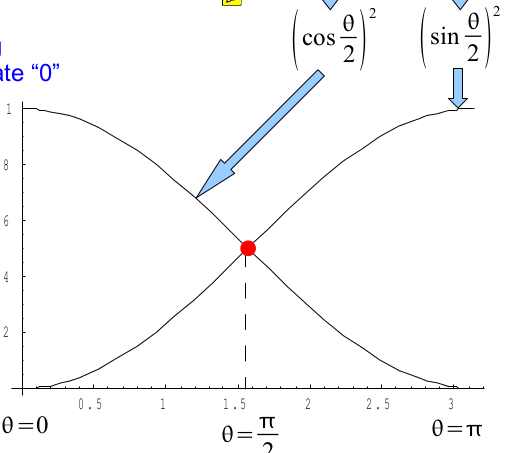
\includegraphics[width=0.8\textwidth,height=10\baselineskip,keepaspectratio]{ch3/image4} 
	\caption{Champ proche et champ lointain} 
	\label{fig:champproloin}
\end{figure}
\begin{figure}[H] 
	\centering 
	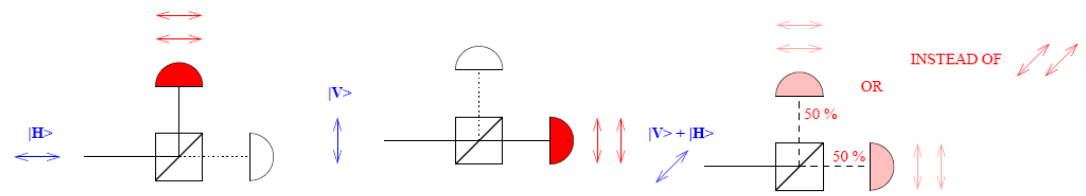
\includegraphics[width=0.8\textwidth,height=10\baselineskip,keepaspectratio]{ch3/image5} 
	\caption{Type de couplages}
	\label{fig:typcouplage} 
\end{figure}
Quelques exemples de parasites sont cités slide 46.
\subsection{Parasites rayonnés}
\subsubsection{Couplage capacitif}
Les charges portées par un conducteur induisent des charges opposées (\(\Rightarrow\) courant) dans un autre conducteur via le champ électrostatique \(E\). Existe entre toute paire de conducteurs et est modélisé par une capacité parasite entre ces conducteurs. À prendre en compte dans le domaine du \textbf{champ proche} (\(L<\lambda/2\pi\)). Ex.: pistes proches ou superposée dans les circuits imprimés, les bus, etc.\bigbreak

\(\Rightarrow\) éviter les lignes parallèles, éloigner le plus possible les fils les uns des autres afin de réduire les capacités parasites ou disposer d'un blindage électrostatique (décrit plus bas).

Un cas particulier existe, les \textbf{décharges électrostatiques}:
\begin{description}
	\item[définition] claquage de l'isolant entre les armatures du condensateur parasite lorsque le champs électrique devient trop important
	\item[exemple] tapis, vêtement en laine, éclair en cas d'orage, claquage de l'oxyde de grille dans les circuits MOS
	\item[contre-mesure] mise à la terre des dispositifs/utilisateurs pour les décharger et éviter l'accumulation de charge, intégrer un dispositifs de dissipation de puissance (parasurtenseurs, décrit plus bas)
\end{description}
Un exemple de dispositif permettant d'empêcher l'accumulation de charge se trouve \autoref{fig:dispdechdio}. La diode protectrice protège le circuit en aval en permettant le passage du courant parasite en cas de surtension.
\begin{figure}[H] 
	\centering
	\begin{circuitikz}
	\draw (0,0) node[left]{\SI{0}{\volt}} to[short] (4,0) to[open] (4,1) to[short] (0,1) node[left]{\SI{5}{\volt}};
	\draw (2,0) to[sDo,l_=\SI{6}{\volt}] (2,1);
	\end{circuitikz}
	\caption{Dispositif de décharge} 
	\label{fig:dispdechdio}
\end{figure}
\subsubsection{Couplage inductif}
Un champ magnétique variable induit dans un conducteur une f.e.m. qui tend à s'opposer à cette variation (loi de Lenz). Existe en théorie dans toute paire de conducteur et est modélisé par une inductance mutuelle parasite entre ces conducteurs. À prendre en compte dans le domaine du \textbf{champ proche} (\(L<\lambda/2\pi\)). Ex.: lignes de signal (téléphone, instrumentation) entre elles ou placées à coté d'une ligne d'alimentation/moteur électrique etc.\bigbreak

Il faut donc éloigner les sources de champ magnétique, minimiser la surface offerte au champ magnétique extérieure (réduire l'inductance mutuelle en jouant sur l'orientation spatiale ou sur la surface de la boucle, en tressant les câbles par exemple), implémenter un blindage magnétique (décris plus bas).\\
Mode de couplage le plus répandu, toute boucle formée de conducteur est une victime potentielle. Phénomène d'autant plus critique que la fréquence est élevée. 

Un cas particulier, les \textbf{câbles de transmission}. Ceux-ci forment une boucle et sont donc des victimes privilégiés. Il existe quelques contre-mesures:
\begin{itemize}
	\item réduire la surface de la boucle:
	\begin{itemize}
		\item réduire la longueur des câbles
		\item rapprocher les conducteurs aller et retour
		\item torsader les fils d'amenée et de retour. Si au-delà des quelques \si{\mega\hertz}, passer au câble coaxial (mutuelle nulle).
	\end{itemize}
	\item câbles blindés
	\item passer à une transmission ayant une meilleur immunité:
	\begin{itemize}
		\item boucle de courant (si la transmission est en courant, il n'y a pas d'impact)
		\item porter l'information sur la fréquence
		\item passer au numérique
		\item code détecteurs/correcteurs d'erreur
	\end{itemize}
\end{itemize}

\subsubsection{Couplage électromagnétique}
Dans le domaine du \textbf{champ lointain} (\(L>\lambda/2\pi\)), \(E\) et \(H\) coexistent sous forme d'une onde plane. Tout conducteur peut se comporter comme une antenne réceptrice parasite à l'onde plane. C'est d'autant plus critique que la fréquence est élevée. Ex.: GSM dans les hôpitaux ou les avions etc.\bigbreak

Il faut donc limiter la source d'émission, implémenter un blindage EM (plus bas), designer le circuit récepteur, ou  utiliser un dispositif optique (comme la fibre optique).
\subsubsection{Blindage}
\underline{\textit{Blindage électrostatique} (champ proche)}: utiliser un matériau conducteur dont le potentiel est imposé. Ceci offre un chemin de retour pour le courant parasite et évite de modifier le potentiel du circuit victime. Le plus souvent, c'est une mise à la terre via une impédance faible. Ex.: blindage complet (boîtier) ou \autoref{fig:blindelectrostat}.\\
Il faut bien comprendre ici qu'au lieu de réduire la capacité parasite, nous interposons des conducteurs supplémentaires dont le potentiel est fixé. De plus, rien ne nous interdit de fixer un potentiel différent de la masse/terre (\SI{0}{\volt})
\begin{figure}[H] 
	\centering 
	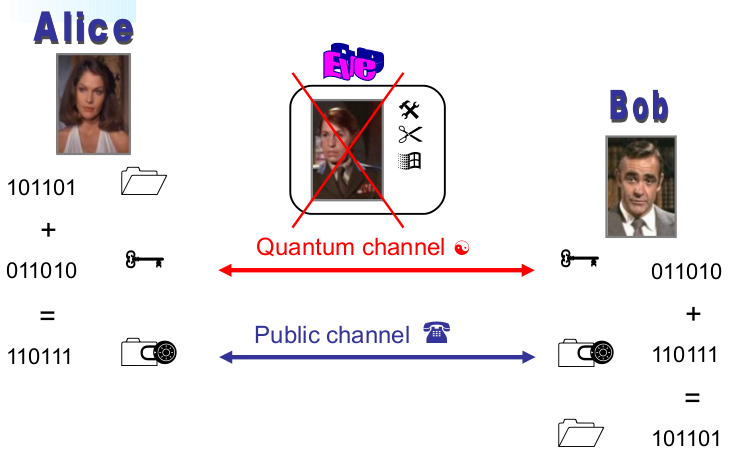
\includegraphics[width=0.7\textwidth,height=10\baselineskip,keepaspectratio]{ch3/image6} 
	\caption{Forme de blindage électrostatique}
	\label{fig:blindelectrostat}
\end{figure}
\begin{figure}[H] 
	\centering 
	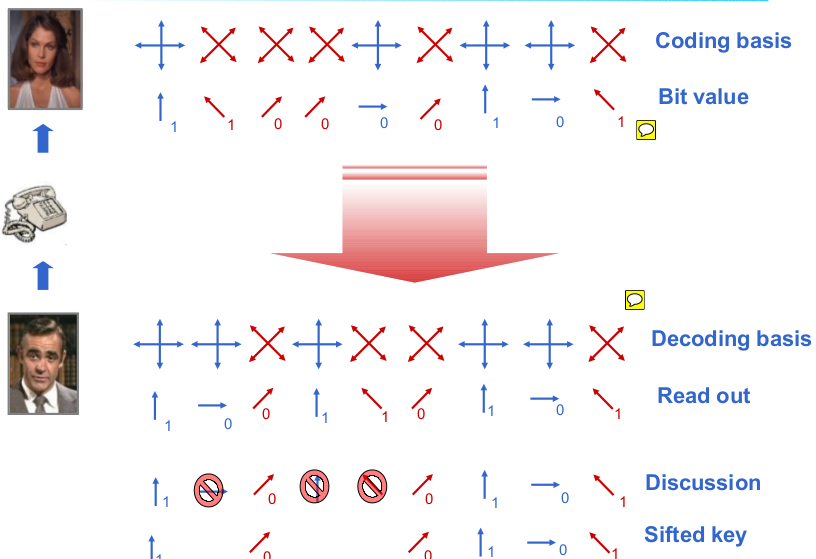
\includegraphics[width=0.8\textwidth,height=10\baselineskip,keepaspectratio]{ch3/image7} 
	\caption{Blindage électrostatique}
\end{figure}
\underline{\textit{Blindage magnétique} (champ proche)}: ici nous avons 2 cas:
\begin{itemize}
	\item champ BF: matériau ferromagnétique (\(\mu\) élevé). Il dévie les lignes de champ magnétique, mais il faut faire attention à la saturation \(\Rightarrow\) grande épaisseur du ferromagnétique (mais cher et lourd) (\autoref{fig:blindmagn}).
	\item champ HF: matériau conducteur (non ferromagnétique). les courants de Foucault induits dans le blindage s'opposent à la pénétration du champ extérieur.
\end{itemize}
\begin{figure}[H] 
	\centering 
	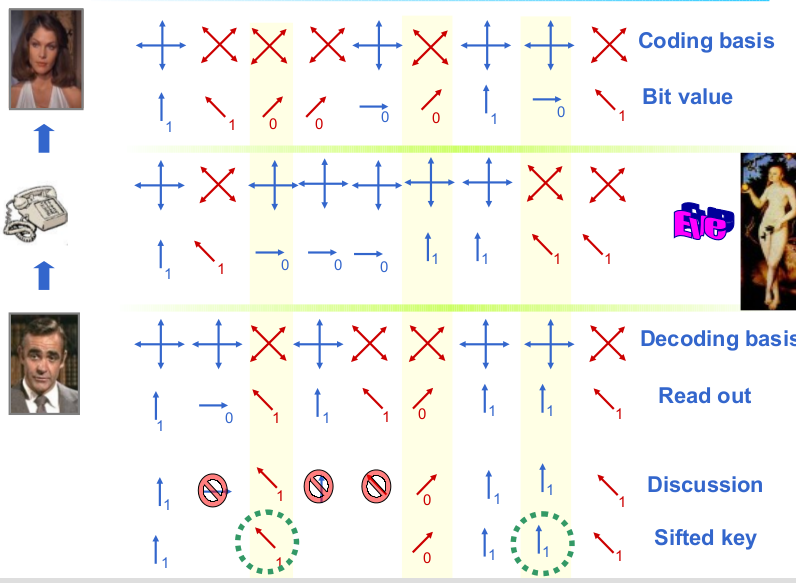
\includegraphics[height=4\baselineskip]{ch3/image8} 
	\caption{Blindage ferromagnétique}
	\label{fig:blindmagn}
\end{figure}

\underline{\textit{Blindage EM} (champ lointain)}: utiliser un matériau conducteur qui supprimera le champ perturbateur par un champ opposé induit (courant de Foucault). Typiquement, une cage de Faraday. Néanmoins, il nécessite de faire rentrer les lignes de signal et d'alimentation (coucou couplage inductif) et la moindre ouverture réduit l'efficacité du blindage \(\Rightarrow\) construction très délicate.\bigbreak

\underline{\textit{Remarques générales}}: Les blindages concerne tout autant les câbles de transmission que les boîtiers (capteur, instrumentation). De plus la connections des blindages de câbles n'est pas trivial.
\subsection{Parasites conduits}
\subsubsection{Introduction}
Commençons pas définir ce qu'est un \emph{couplage galvanique}:
\begin{description}
	\item[définition] transmission d'un signal perturbateur entre la source de ce signal et le dispositif victime \emph{via un conducteur commun}.
\end{description}
Ceci concerne autant les lignes de signal que les alims/masse/terre et le simple fait de brancher 2 appareils sur le réseau électrique établit un couplage galvanique. Comme par exemple 2 appareils à \SI{220}{\volt} dans 2 pièces différentes, connectés à la masse. Si l'un demande en puissance, cela fait baisser la tension dans tout le circuit. Il existe 2 origines distinctes:
\begin{enumerate}
	\item le conducteur commun (idéal) transmet un signal parasite issu d'un autre équipement (comme parasite transmis via les lignes d'alimentation à cause de la foudre).
	\item le conducteur commun n'est pas équipotentiel \(\Rightarrow\) la circulation d'un courant sur ce conducteur génère des f.e.m. parasites.
\end{enumerate}
Ces 2 origines sont bien évidement cumulables. Il existe 2 niveaux de conséquences:
\begin{enumerate}
	\item dégrade le signal (superposition du signal utile et parasite, si sur alim \(\rightarrow\) mauvais fonctionnement du circuit).
	\item détruit l'équipement (surtension (claquage électrostatique) ou surpuissance (destruction par échauffement)).
\end{enumerate}
Remarquons que tout parasite rayonné devient f.e.m. ou courant sur un conducteur et donc que les conséquences sont aussi valables pour les parasites rayonnés en amont.
\subsubsection{Contre-mesures}
Il existe 3 contre-mesures générales:
\begin{enumerate}
	\item Contre les parasites conduits issus d'autres équipement:
	\begin{itemize}
		\item filtre passe-bas pour le spectre étendu, filtre réjecteur de fréquence pour le spectre étroit
		\item équilibrer (rendre le circuit plus symétrique, voir plus bas)
	\end{itemize}
 \hspace*{\dimexpr\linewidth-\textwidth\relax}%
 \begin{minipage}[t]{\textwidth}%
 	Néanmoins, il n'est pas trivial de réaliser le filtre, nous pouvons utiliser un filtre passif (capa et inductance) ou actif (passif + AOP), en mode commun ou différentiel.
 \end{minipage} 
	\item Contre les parasites générés par l'impédance des connexions:
	\begin{itemize}
		\item design des connexions (\(\searrow\) longueur + \(\nearrow\) section conductrice \(= \searrow\) impédance)
		\item connecter judicieusement les alimentations et les masses:
		\begin{enumerate}
			\item éviter les chemins communs \(\Rightarrow\) câblages en étoile
			\item séparer alimentations de signaux à fréquence et/ou puissance \(\neq\)
		\end{enumerate}	
	\end{itemize}
	\item Contre la destruction des équipement par surtension/surpuissance \(\Rightarrow\) parasurtenseurs, dont le principe est de limiter la tension  et ayant la capacité de dissiper l'énergie excédentaire:
	\begin{itemize}
		\item diodes Zener utilisée en avalanche (protection)
		\item varistance (résistance non linéaire, \(\nearrow\) tension \(= \searrow\) résistance)
		\item éclateurs (tube à gaz dissipant temporairement l'énergie via un arc électrique)
	\end{itemize}
\end{enumerate}
\underline{\textit{Exemple} (flemme)}:
\begin{figure}[H] 
	\centering 
	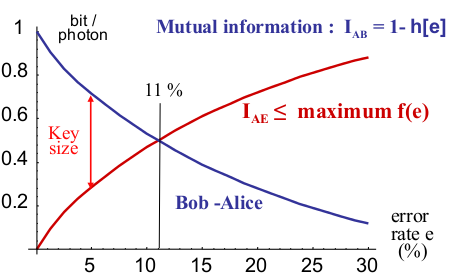
\includegraphics[width=0.8\textwidth,height=10\baselineskip,keepaspectratio]{ch3/image9} 
	\caption{Circuit électronique initial} 
\end{figure}
A première vue, les fils ou pistes d'alimentation sont des équipotentielles. En réalité, il existe souvent une distance de plusieurs centimètres ou dizaines de centimètres entre les bornes d'alimentation d'une carte électronique et le circuit intégré le plus éloigné.\\
L'impédance de ces connections joue un rôle non négligeable:
\begin{itemize}
\item la chute de tension ohmique due à la résistance des connections (l'épaisseur des piste est très faible: de l'ordre de \SI{30}{\micro\meter}) parcourue par le courant moyen.
\item les fluctuations de tension liées aux variations de courant importantes (basculement de portes, charge de capacités parasites, "réveil" d'un circuit CMOS) sur l'inductance des connections \(\rightarrow\) peuvent faire sortir l'alimentation de sa plage normale.
\end{itemize}
\begin{figure}[H] 
	\centering 
	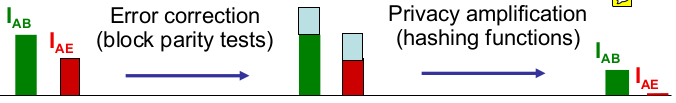
\includegraphics[width=0.8\textwidth,height=10\baselineskip,keepaspectratio]{ch3/image10} 
	\caption{Circuit électronique final} 
\end{figure}
Les améliorations les plus courantes de l'alimentation sont
\begin{itemize}
\item l'utilisation de fils de plus forte section ou de pistes plus larges (quelques \si{\milli\meter}) ou de circuits multi-couches (permettant d'inclure plan de masse et plan d'alimentation)
\item les condensateurs de découplage sous forme
\begin{itemize}
	\item d'un condensateur électrolytique (généralement quelques \si{\micro\farad}) 
	\item d'un ensemble de condensateurs de très bonne qualité disséminés sur toute la carte, le plus près possible des pattes d'alimentation de chaque gros circuit intégré et de chaque groupe de petits circuits

\end{itemize}
\item une diode Zener (protection contre les surtensions)
\end{itemize}
Les condensateurs constituent des sources de tension localisée (à très court terme) vis-à-vis des impulsions de courant consommées par les circuits intégrés.\bigbreak

Le mot "découplage" qualifie le fait que les variations de consommation (composante alternative) propres du circuit ne sont pas vues par les fils d'alimentation, qui ne véhiculent que la composante continue (moyenne). Les inductances parasites du câblage ont donc beaucoup moins d'influence.\bigbreak

La diode Zener permet d'écrêter les surtensions transitoires. Si celles-ci sont répétitives, l'absorption d'énergie par la Zener peut excéder ses capacités de refroidissement et la détruire. En cas de tension d'entrée trop importante, la Zener va également surchauffer et fondre, généralement en court-circuit, ce qui protégera les circuits coûteux en aval.
\subsubsection{Isolation galvanique}
\begin{description}
	\item[définition] coupure de tout lien galvanique entre 2 parties du montage
	\item[moyen] couplage magnétique (transformateur) et couplage optique (optocoupleur, fibre optique)
\end{description}
C'est souvent nécessaire pour des raisons de protection des utilisateurs et des équipements (sécurité). Le but est de faire passer de la puissance/info d'une autre manière que via de l'électricité.
\iffalse \subsection{Compatibilité électromagnétique}
\begin{description}
	\item[définition] discipline ayant pour but d'analyser et de résoudre l'ensemble des problèmes de parasitage EM d'un équipement par un autre
\end{description}
C'est une discipline de plus en plus importante en raison de la multiplications des équipement électroniques. Il existe des normes stricte depuis les années 90. On définit:
\begin{description}
	\item[CEM/EMC] compatibilité EM
	\item[IEM/EMI] interférence EM
\end{description}
\subsection{Notions embrassées par la CEM}
les normes CEM, les types de couplages, les imperfections des composants (passif et surtout actifs car sources de perturbations), les boîtiers et blindages, le câblage, le routage des pistes dans les circuits imprimés (surtout masse et alim) et « tous les effets du second ordre ».
\subsection{Exemple: alimentation à découpage}
Exemple slide 81--85.\fi
\section{Câblage et connexions}
\subsection{Référence d'un signal}
Rappel sur tension et masse slide 88. Nous ajoutons quelques subtilités:
\begin{enumerate}
	\item impédance de masse: en pratique la "masse" d'un montage peut être un conducteur ayant une certaine extension physique \(\Rightarrow\) impédance \(\neq 0 \Rightarrow\) lorsque parcouru par un courant, pas équipotentiel \(\Rightarrow\) plus vraiment une masse (f.e.m. parasite)
	\item plusieurs montages: les masses de différents montages sont à priori pas au même potentiel (pas connecté ou connecté via des impédance \(\neq 0\))
\end{enumerate}
Pour rappel, la mise à terre est une connexion d'un conducteur au potentiel de la terre (sol) afin d'assurer la protection des utilisateurs et des équipements (le réseau de terre doit avoir l'impédance la plus faible possible). La masse (référence) et la terre (protection) ne sont pas forcément connectées.\bigbreak

On définit les appareils:
\begin{description}
	\item[flottants] aucune des 2 bornes du signal (entrée ou sortie) n'est connectée à la terre (appareils portatifs, appareils sur réseau à 3 bornes)
	\item[non flottants] masse = terre
\end{description}
\subsection{Montage "single-ended"}
\subsubsection{Cas idéal}
Un montage "single-ended" possèdent les caractéristiques suivantes:
\begin{itemize}
\item un amplificateur "single-ended" (= asymétrique) comme un (non-)inverseur, suiveur à AOP. Au niveau multiplexage, il faut \(N+1\) fils pour \(N\) signaux. \item La référence du capteur = la référence de l'instrumentation
\end{itemize} 
Dans le cas théorique \(V_{in}=e_s\) (donc pas de parasites).
\begin{figure}[H] 
	\centering 
	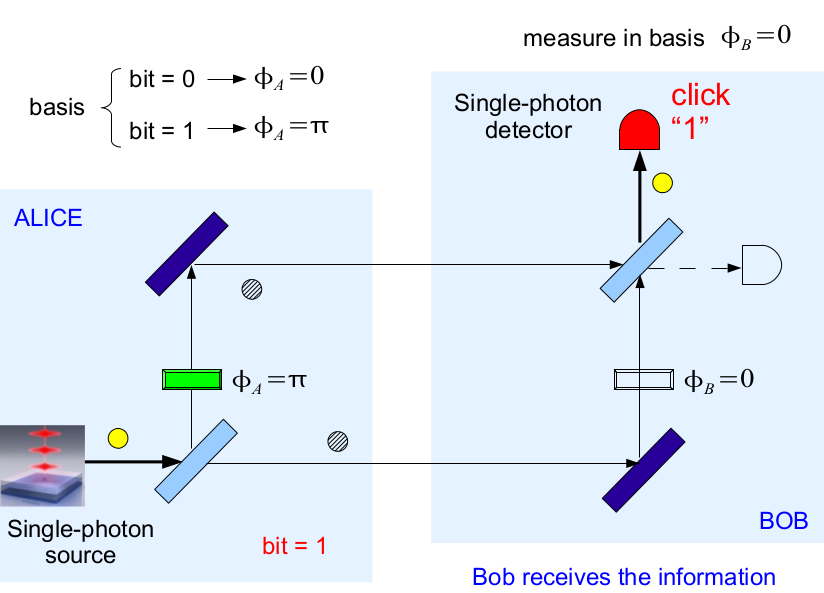
\includegraphics[width=0.8\textwidth,height=10\baselineskip,keepaspectratio]{ch3/image11} 
	\caption{Single-ended (idéal)} 
\end{figure}
\subsubsection{Cas réel}
Dans le cas réel, une source parasite \(e_p\) vient s'ajouter car il existe une impédance de masse non négligeable et des parasites induits dans la boucle. Il en résulte \(V_{in} = e_s + e_p\) et donc un signal dégradé.
\begin{figure}[H]
	\centering 
	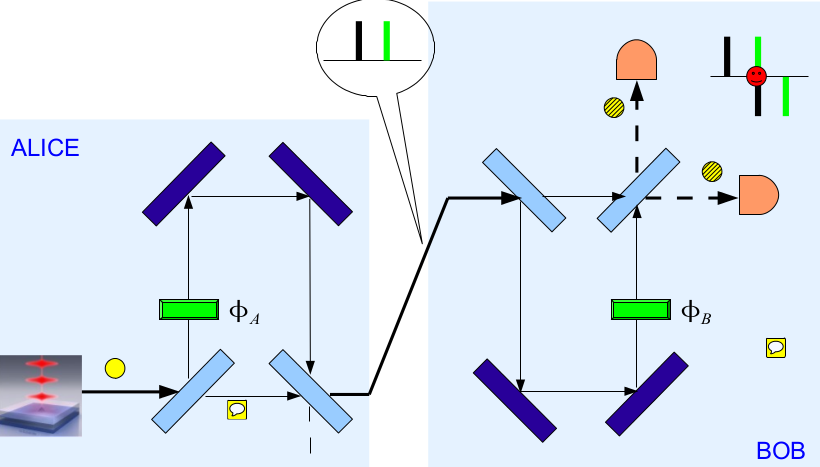
\includegraphics[width=0.8\textwidth,height=10\baselineskip,keepaspectratio]{ch3/image12} 
	\caption{Single-ended (réel)} 
\end{figure}
\(\Rightarrow\) éviter les montages "single-ended". Sauf si la chute de tension sur l'impédance de masse ET les f.e.m induites sont négligeables, comme pour:
\begin{itemize}
	\item un capteur proche de l'ampli
	\item un capteur éloigné mais isolé de son environnement et sa masse est ramenée à l'ampli par une connexion d'impédance négligeable
\end{itemize}
\subsection{Montage différentiel}
\begin{figure}[H] 
	\centering 
	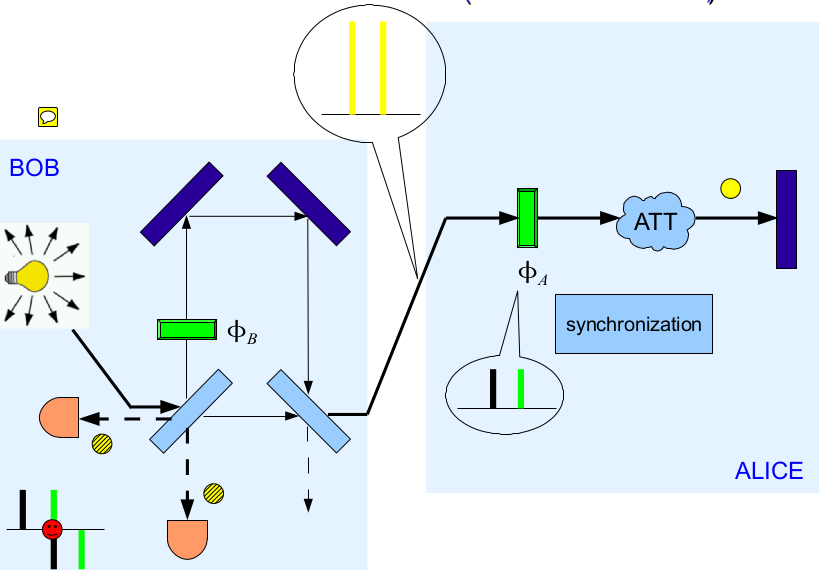
\includegraphics[width=0.8\textwidth,height=10\baselineskip,keepaspectratio]{ch3/image13} 
	\caption{Montage différentiel} 
\end{figure}
Dans ce montage, nous avons:
\begin{itemize}
		\item {\makebox[8cm]{tension d'entrée de l'ampli différentiel\hfill} \(V^-=e_p\qquad V^+=e_s+e_p\)} 
		\item {\makebox[8cm]{tension différentielle\hfill} \(V_{md} = V^+-V^-=e_s\)} 
		\item {\makebox[8cm]{tension de mode commun (parasites)\hfill} \(V_{mc}=\frac{V^++V^-}{2}=e_p+\frac{e_s}{2}\)} 
		\item {\makebox[8cm]{tension de sortie\hfill} \(V_{out}=A_{md}V_{md}+A_{mc}V_{mc}\)} 
		\item {\makebox[8cm]{taux de réjection en mode commum\hfill} \(\text{CMRR} = \frac{A_{md}}{A_{mc}}\)} 
\end{itemize}
Il faut donc maximiser le CMRR (common mode rejection ratio). On en déduit les avantages et inconvénients suivants:
\begin{description}
	\item[avantages]:
	\begin{itemize}
		\item les parasites de mode commun, les parasites par couplage galvanique et les autres parasites induits en mode commun sont rejetés
		\item signal dont aucune des bornes ne peut être considérée comme une masse (même imparfaite). ex: tension de déséquilibre d'un pont de Wheatstone ou un montage porté à une tension élevée.
	\end{itemize}
	\item [inconvénients]:
	\begin{itemize}
		\item les parasites de mode différentiel sont toujours amplifiés
		\item liaison \(2N\) (ou \(2N+1\)) fils pour \(N\) signaux
	\end{itemize}
\end{description}
\underline{\textit{Remarques}}: en instrumentation, la tension de mode commun est souvent du même ordre de grandeur  voir plus élevée que la tension différentielle. On essayera de faire apparaître les parasites sous forme de tension en mode commun car elles seront rejetés (pas entièrement, dépend du CMRR). Hélas, un bon CMRR ne suffit pas.
\begin{figure}[H] 
	\centering 
	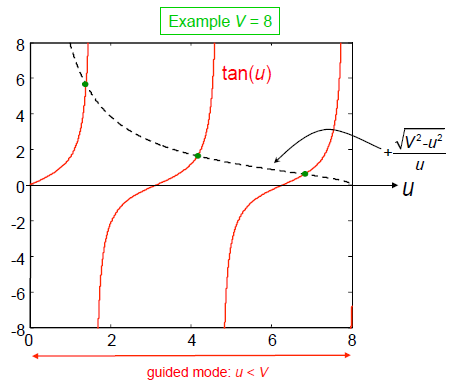
\includegraphics[width=0.8\textwidth,height=10\baselineskip,keepaspectratio]{ch3/image14} 
\end{figure}
Pour un multiplexeur, les deux montages s'implémentent comme illustré à la \autoref{fig:multmont}
\begin{figure}[H]
	\centering
	\subfigure[Single-ended]{\label{fig:multsing}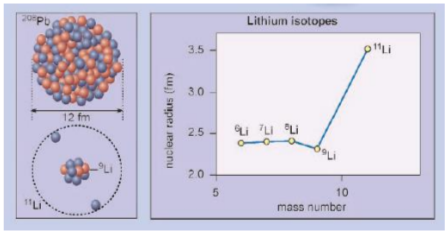
\includegraphics[width=0.4\textwidth]{ch3/image15}}
	\subfigure[Différentiel]{\label{fig:mutldiff}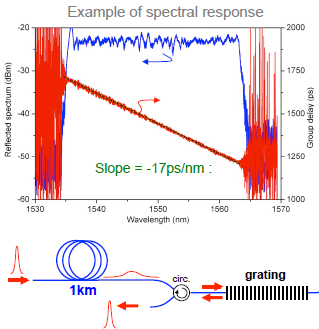
\includegraphics[height=15\baselineskip]{ch3/image16}}
	\caption{Implémentation avec un multiplexeur}
	\label{fig:multmont}
\end{figure}
\subsection{Symétrie des voies d'amenée}
\subsubsection{Déséquilibre série}
\begin{figure}[H] 
	\centering 
	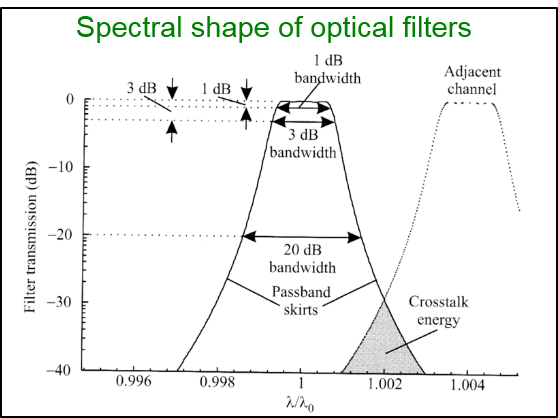
\includegraphics[width=0.8\textwidth,height=10\baselineskip,keepaspectratio]{ch3/image17} 
	\caption{Déséquilibre série} 
\end{figure}
Soit \(Z_1, Z_2\) les impédances série des voies d'amenée (souvent résistif) et soit un ampli différentiel ayant comme impédances d'entrée:
\begin{itemize}
	\item 1 impédance différentielle \(Z_d\) (hyp: \(\infty\))
	\item 2 impédances mode commun \(Z_{mc}\) (hyp: identiques)
\end{itemize}
Souvent \(Z_{mc} = \SI{e10}{\ohm}\)  \(\parallelsum\) capa en \si{\pico\farad} \(\Rightarrow \text{ passe-bas }f_c\approx \SI{10}{\hertz}\). Nous avons donc:
\[v_d = v_2-v_1\qquad v_d'=v^+-v^-\qquad v_{mc}=\frac{v_1+v_2}{2}\qquad v_{mc}'=\frac{v^++v^-}{2}\]
Les tensions à l'entrée de l'ampli sont:
\[v^-=\frac{Z_{mc}}{Z_1+Z_{mc}}v_1\qquad v^+=\frac{Z_{mc}}{Z_2+Z_{mc}}v_2\]
en faisant l'hypothèse que \(Z_{mc}\gg Z_1, Z_2\):
\[v_{mc}'\approx v_{mc}\qquad v_d'=v_d+\frac{Z_1-Z_2}{Z_{mc}}v_{mc}\]
La tension différentielle est polluée par une fraction de la tension de mode commun, fraction d'autant plus importante que \(Z_1\text{ et }Z_2\) sont \(\neq\) et que \(Z_{mc}\) est petit. Tout déséquilibre engendrera une dégradation du CMRR. En particulier, il faut que \(R_1=R_2\) pour une bonne réjection des tensions de mode commun continues et basse fréquence.
\subsubsection{Déséquilibre parallèle}
\begin{figure}[H] 
	\centering 
	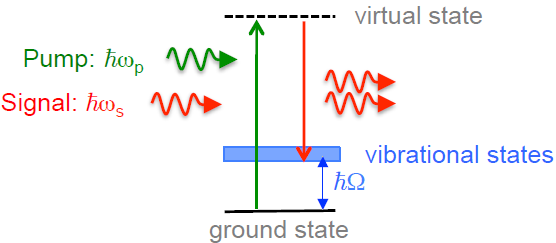
\includegraphics[width=0.8\textwidth,height=10\baselineskip,keepaspectratio]{ch3/image18} 
	\caption{Désiquilibre parallèle} 
\end{figure}
On ajoute maintenant \(C_1', C_2'\) des capa parasites \(\parallelsum\) venant s'ajouter aux 2 capas \(C_{mc}\) de l'ampli. Nous avons donc:
\[C_1=C_1'+C_{mc}\qquad C_2=C_2'+C_{mc}\] 
\begin{figure}[H] 
	\centering 
	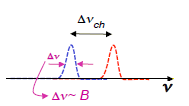
\includegraphics[width=0.8\textwidth,height=10\baselineskip,keepaspectratio]{ch3/image19}
\end{figure}
En supposant toujours que \(Z_d\gg\)
\[v^-=\frac{(R_{mc} \parallelsum C_1)}{R_1+(R_{mc} \parallelsum C_1)}\qquad v^+=\frac{(R_{mc} \parallelsum C_2)}{R_2+(R_{mc} \parallelsum C_2)}\] 
Dans la gamme de fréquence \(\frac{1}{R_{mc}C_1},\frac{1}{R_{mc}C_2}\ll\omega_{mc}\ll\frac{1}{R_1C_1},\frac{1}{R_2C_2}\) on a:
\[v_{mc}'\approx v_{mc}\qquad v_d'=v_d+j\omega(R_1C_1-R_2C_2)v_{mc}\]
La tension différentielle est polluée par une fraction de la tension de mode commun, fraction d'autant plus importante que \(C_1\text{ et }C_2\) sont différentes, mais cette fois, c'est surtout pour les fréquences plus élevées.\bigbreak

En pratique, \(C_1'\text{ et }C_2'\) sont des capas parasites qui existent vis-à-vis du blindage électrostatique des voies d'amenée, alors que précédemment, on a fait l'hypothèse d'être à la masse. En portant le blindage à la tension de mode commun \(v_{mc}\), on annule la tension différentielle parasite due au déséquilibre de \(C_1', C_2'\), c'est la \emph{garde}.
\begin{figure}[H] 
	\centering 
	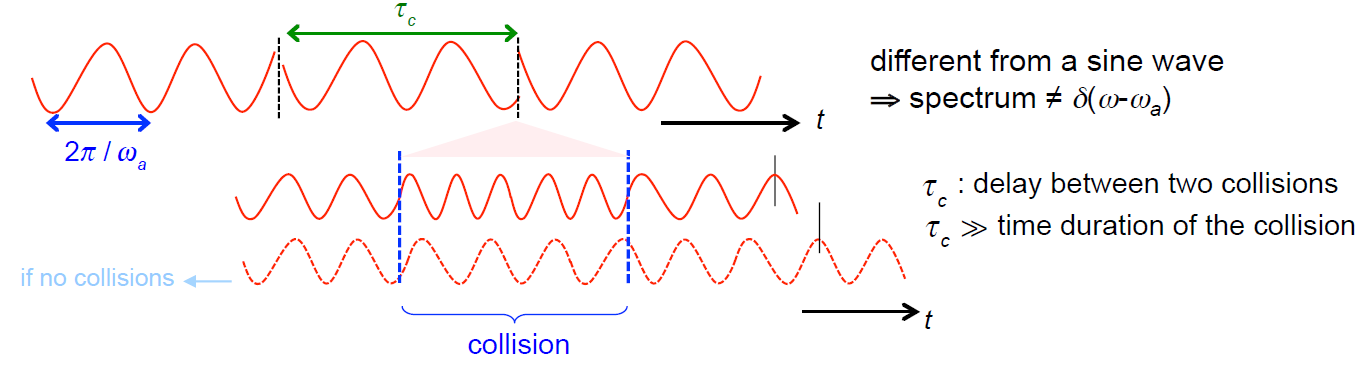
\includegraphics[width=0.7\textwidth,height=10\baselineskip,keepaspectratio]{ch3/image20} 
	\caption{Désiquilibre parallèle: garde} 
\end{figure}
\subsection{Montage différentiel avec \texorpdfstring{\(v_{mc}\)}{tension de mode commun} élevée}\label{subsec:montdiffvmcgrand}
Avant, on avait \(2N+1\) conducteurs et un \(v_{mc}\) relativement faible (les 2 références restaient proches). Dans le cas d'un source flottante (pas connectée à la référence) on a:
\begin{itemize}
	\item \(2N\) conducteurs
	\item tension de mode commun quelconque et variable dans le temps (AC + DC)
\end{itemize}
Une très mauvaise idée car nous avons une source de perturbations importante qui risque de détruite le matériel par surtension.

N.B.: vérifier la capa de l'ampli à tenir la tension de mode commun (\!?).
\subsubsection{1\up{ère} solution: bias resistor pour source flottante}
Il faut limiter la tension de mode commun, donc soit on utilise \(2N+1\) conducteurs (donc retour au cas précédent) soit on utilise des résistances offrant une liaison galvanique de haute impédance ("bias resistor):
\begin{itemize}
	\item meilleur symétrie que \(2N+1\) conducteurs
	\item valeur suffisamment élevée pour ne pas imposer le potentiel des entrées
	\item mais suffisamment faible pour éviter que la tension de mode commun soit trop éloignée de la référence de l’instrumentation
	\item typiquement: \SI{10}{\kilo\ohm} à \SI{100}{\kilo\ohm}
\end{itemize}
\begin{figure}[H] 
	\centering 
	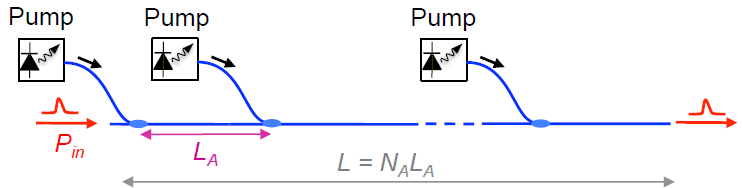
\includegraphics[width=0.7\textwidth,height=10\baselineskip,keepaspectratio]{ch3/image21} 
	\caption{bias resistor pour source flottante} 
\end{figure}
\subsubsection{2\up{ème} solution: ampli d'isolation}
\begin{figure}[H] 
	\centering 
	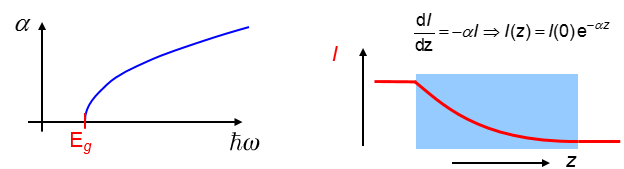
\includegraphics[width=0.7\textwidth,height=10\baselineskip,keepaspectratio]{ch3/image22} 
	\caption{Ampli d'isolation} 
\end{figure}
Comme ceci l'instrumentation au potentiel du capteur possède sa propre alimentation et donc pas de mode commun.
\subsection{Conclusion}
Il y a 3 cas à distinguer:
\begin{enumerate}
	\item les références sont identiques:
	\begin{itemize}
		\item différence de potentiel nulle ou négligeable: c'est l'exception, les f.e.m. par impédance de masse et parasites sont négligeables, la référence est indifféremment la masse ou la terre. Un simple montage asymétrique convient.
	\end{itemize}
	\item les références sont proches:
	\begin{itemize}
		\item tension de mode commun "faible": typiquement un cas \(2N+1\) fils. Un montage différentiel "simple" convient (il faut vérifier la limite de l'ampli vis-à-vis du mode commun)
	\end{itemize}
	\item les références sont éloignées:
	\begin{itemize}
		\item tension de mode commun élevée (ou quelconque): capteur flottant et porté à un potentiel élevé. Il faut limiter le mode commun \(\Rightarrow 2N+1\) fil ou bias resistors ou reprendre le mode commun grâce à l'ampli d'isolation.
	\end{itemize}
\end{enumerate}
De plus, au niveau de la boucle différentielle, les mesures classiques pour limiter les parasites sont le câble torsadé ou coaxial, le blindage des câbles (complexe), etc.
\section{Transmission des signaux}
\subsection{Introduction}
La majorité des transmissions des signaux se font par tension analogique, le montage différentiel ne résout pas tout (il résout surtout le couplage galvanique). Pour les environnements très parasités et/ou longues distances, nous aurons recours à des transmissions par boucle de courant, par fréquence, par signal optique ou des transmission numérique.
\subsubsection{Inconvénients d'une transmission en tension}
Illustrons une transmission en tension (\autoref{fig:transmtension}). Nous aurons donc \(R_{in}\) élevé et \(R_{out}\) faible (adaptation d'impédance en tension) mais la liaison à distance possède une \(R_{\text{fils}}\) non négligeable. La sortie obtenue est donc 
\[v = e\frac{R_{in}}{R_{out}+R_{in}+R_{\text{fils}}}<e\]
On a donc un affaiblissement du signal, 1\up{er} inconvénient.\\
Prenons le cas maintenant d'une tension parasite par couplage magnétique (\autoref{fig:transmtensionpara})
\[v = (e_s+e_p)\frac{R_{in}}{R_{out}+R_{in}}\]
Le parasite induit se superpose au signal, 2\up{ème} inconvénient
\begin{figure}[H] 
	\centering 
	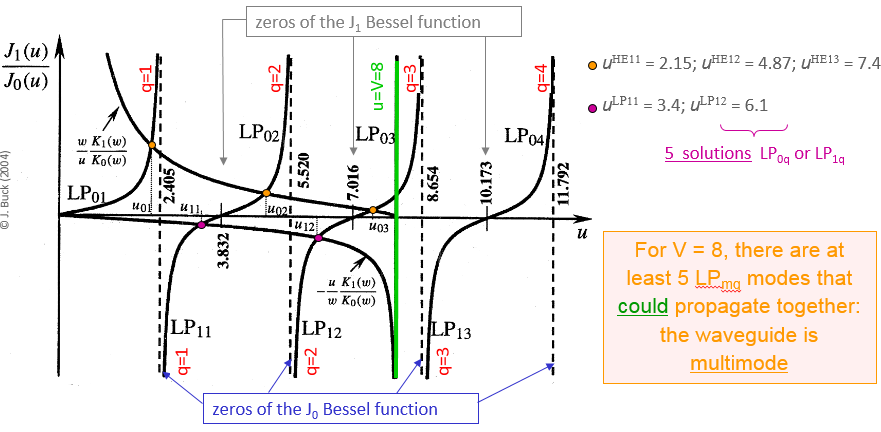
\includegraphics[width=0.6\textwidth,height=10\baselineskip,keepaspectratio]{ch3/image23} 
	\caption{Transmission en tension: résistance de ligne} 
	\label{fig:transmtension}
\end{figure}
\begin{figure}[H] 
	\centering 
	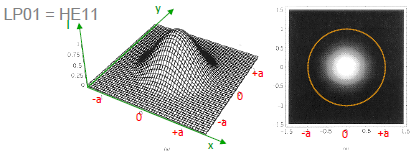
\includegraphics[width=0.6\textwidth,height=10\baselineskip,keepaspectratio]{ch3/image24} 
	\caption{Transmission en tension: parasite de ligne par couplage magnétique} 
	\label{fig:transmtensionpara}
\end{figure}
\subsection{Boucle de courant}
Le but est de passer l'information non plus par une tension, mais par un courant. Il est en pratique plus facile d'obtenir \(R_{out}\) (commande en courant) élevée que \(R_{in}\) élevée (commande en tension). Dans le cas de la \autoref{fig:transcourant}, nous obtenons \((R_{in}+R_{fils})i = R_{out}(i_s-i)\) et donc
\[i=\frac{R_{out}}{R_{out}+R_{in}+R_{fils}}i_s\]
L'affaiblissement du signal est beaucoup plus faible qu'en tension (car plus facile d'obtenir un \(R_{out}\) élevée qu'un \(R_{in}\) élevée).\\
Avec le couplage magnétique (\autoref{fig:transcourantpara}):
\[i_p=\frac{e_p}{R_{out}+R_{in}}\]
Comme \(R_{out}\) élevée, \(i_p\ll i_s \Rightarrow\) bonne immunité aux parasites magnétiques.\\
Plusieurs avantages:
\begin{itemize}
	\item bien pour transmission longue distance (\SI{1}{\kilo\meter} ou plus) car l'impédance des fils influence peu le courant
	\item bonne immunité aux f.e.m. induites car les valeurs idéales de \(R_{out}\text{ et }R_{in}\) sont plus facile à approcher en commande en courant qu'en commande en tension
	\item On peut utiliser un courant \(\neq0\) pour représenter la valeur 0 afin de détecter la rupture de la liaison
\end{itemize}
\begin{figure}[H] 
	\centering 
	\includegraphics[width=0.6\textwidth,height=10\baselineskip,keepaspectratio]{ch3/image35} 
	\caption{Transmission en courant: résistance de ligne} 
	\label{fig:transcourant}
\end{figure}
\begin{figure}[H] 
	\centering 
	\includegraphics[width=0.6\textwidth,height=10\baselineskip,keepaspectratio]{ch3/image36} 
	\caption{Transmission en courant: parasite de ligne par couplage magnétique} 
	\label{fig:transcourantpara}
\end{figure}
\section{Câblage de la masse}
On a plusieurs circuits qui partagent la même alimentation et qui doivent s'échanger de l'information, chacun devant être connecté à une référence unique (masse). Comment câbler?
\subsection{Interconnexion des circuits}
Il faut éviter les impédances communes \(\rightarrow\) mettre en étoile \(\rightarrow\) si le PCM à une impédance nulle \(\Rightarrow\) pas de couplage d'impédance
\begin{figure}[H] 
	\centering 
	\includegraphics[width=0.8\textwidth,height=10\baselineskip,keepaspectratio]{ch3/image25} 
	\caption{Interconnexion des circuits en étoile} 
\end{figure} 
\subsection{Câblage de la masse analogique}
\begin{figure}[H] 
	\centering 
	\includegraphics[width=0.6\textwidth,height=10\baselineskip,keepaspectratio]{ch3/image26}
\end{figure}
Dans le cas analogique, que faire ? Étoile ou cascade ?
\subsubsection{Masse en étoile}
\begin{figure}[H] 
	\centering 
	\includegraphics[width=0.8\textwidth,height=10\baselineskip,keepaspectratio]{ch3/image27} 
	\caption{Masse analogique en étoile} 
\end{figure}
\begin{description}
	\item[Avantages] pas d'impédance commune
	\item[Désavantages] longueur des pistes et formation de boucle
\end{description}
\subsubsection{Masse en cascade}
\begin{figure}[H] 
	\centering 
	\includegraphics[width=0.8\textwidth,height=10\baselineskip,keepaspectratio]{ch3/image28} 
	\caption{Masse analogique en cascade (amont)} 
\end{figure}
Dans ce cas-ci, tous les courants passent pas \(R_1 \Rightarrow V_{in}=V_{out}/\num{e4}\) car on amplifie \(V_{in}+ i_iR_1\)!
\begin{figure}[H] 
	\centering 
	\includegraphics[width=0.8\textwidth,height=10\baselineskip,keepaspectratio]{ch3/image29} 
	\caption{Masse analogique en cascade (aval)} 
\end{figure}
Dans ce cas-là, nous avons minimiser les courants dans \(R_1\).
\subsection{Câblage de la masse numérique}
À haute fréquence, l'effet selfique des câbles devient dominant \(\Rightarrow\) pistes à grande impédance et courants passent par capas parasites\(\Rightarrow\) \cancel{masse en étoile} plan de masse (minimise les inductances et les boucles). Le courant suivra le chemin de moindre impédance.
\begin{figure}[H] 
	\centering 
	\includegraphics[width=0.5\textwidth,height=10\baselineskip,keepaspectratio]{ch3/image30} 
	\caption{Plan de masse} 
\end{figure}
\subsection{CAN et CNA}
\begin{figure}[H] 
	\centering 
	\includegraphics[width=0.5\textwidth]{ch3/image31} 
\end{figure}
Dans un CAN/CNA, il y a un faible courant qui circule à travers sa capa parasite.\\
Il faut 2 masses distinctes pour conserver une topologie en étoile et il faut placer le CAN sur le point central de masse
\begin{figure}[H] 
	\centering 
	\includegraphics[width=0.7\textwidth,height=10\baselineskip,keepaspectratio]{ch3/image32} 
\end{figure}
\subsubsection{Câblage des alimentation}
2 problèmes se posent:
\begin{itemize}
	\item Ripple des alimentation à découpage (fluctuation autour de la valeur consigne)
	\item Consommation des différents circuits
\end{itemize}
\begin{figure}[H] 
	\centering 
	\includegraphics[width=0.7\textwidth,height=10\baselineskip,keepaspectratio]{ch3/image33}  
\end{figure}
Il faut mettre une capa a côté du composant, elle jouera le rôle de réservoir de charge. Sachant que la résistance parasite est d'autant plus grande que la capa est grande, on placera une plus petite capa en parallèle dans le cas HF car c'est la résistance qui est gênante.
\begin{figure}[H] 
	\centering 
	\includegraphics[width=0.6\textwidth,height=10\baselineskip,keepaspectratio]{ch3/image34}  
\end{figure}


%%%%%%%%%%%%%%%%%
% Bibliographie %
%%%%%%%%%%%%%%%%%
%\newpage
%\chapter{Bibliographie}
%\nocite{*}
%\printbibliography[heading=none]

%%%%%%%%%%%
% Annexes %
%%%%%%%%%%%
\appendix
%\input{annexes/annexe1.tex}


\end{document}
